\documentclass[12pt]{article}
\usepackage{fullpage}
\usepackage[titletoc,toc,page]{appendix}
\usepackage{setspace}
\usepackage{titlesec}
\usepackage{blindtext}
\usepackage{graphicx}
\usepackage{amssymb}
\usepackage{listings}
\usepackage[table]{xcolor}
\usepackage{wrapfig}
\usepackage{xcolor}
\usepackage[main=greek, english]{babel}
\usepackage[utf8]{inputenc}
\usepackage[labelfont=bf]{caption}
\usepackage{kerkis}
\usepackage{url}
\usepackage{multicol}
\usepackage[titles]{tocloft}
\usepackage[top=2.5cm, bottom=2.5cm, left=2.8cm, right=3cm]{geometry}
\usepackage{pgfplots}
\usepackage{hyperref}

\pgfplotsset{width=15cm ,compat=1.9}
\usepgfplotslibrary{external}
\tikzexternalize[prefix=diagrams/]

\hypersetup{
    colorlinks=true,
    linkcolor=blue,
    filecolor=magenta,      
    urlcolor=cyan,
}


\renewcommand\cftsecfont{\normalfont}
\renewcommand\cftsecpagefont{\normalfont}

\newcommand{\en}[1]{\foreignlanguage{english}{#1}}
\newcommand{\el}[1]{\selectlanguage{greek}{#1}\selectlanguage{english}}

\renewcommand\lstlistingname{\el{Συμβ.}}
\renewcommand\lstlistlistingname{Λίστα Συμβολισμών}
\setlength{\columnsep}{1cm}

\graphicspath{ {./images/} }
\setcounter{secnumdepth}{4}



\titlespacing*{\subsection}
{0pt}{2.5ex plus 1ex minus .2ex}{0.3ex plus .2ex}
\titlespacing*{\subsubsection}
{0pt}{2.5ex plus 1ex minus .2ex}{0.3ex plus .2ex}
\pagenumbering{gobble}

\begin{document}
 \begin{center}
\selectlanguage{greek}

\textsc{ ΠΑΝΕΠΙΣΤΗΜΙΟ ΜΑΚΕΔΟΝΙΑΣ\\[0.3 cm]
ΠΡΟΓΡΑΜΜΑ ΜΕΤΑΠΤΥΧΙΑΚΩΝ ΣΠΟΥΔΩΝ\\[0.3 cm]
ΤΜΗΜΑΤΟΣ ΕΦΑΡΜΟΣΜΕΝΗΣ ΠΛΗΡΟΦΟΡΙΚΗΣ}\\[2.5 cm]
{ \large 
ΠΑΡΑΛΛΗΛΟΣ ΠΡΟΓΡΑΜΜΑΤΙΣΜΟΣ ΜΕ ΧΡΗΣΗ \en{OpenMP}\\[0.4 cm] }
Διπλωματική Εργασία\\[1 cm]
του\\[0.5 cm]
\large
Κοντογιάννη Γεώργιου
\begin{minipage}{0.4\textwidth}
\end{minipage}
\vfill
{\large Θεσσαλονίκη, Οκτώβριος 2020}

 \end{center}
 
\pagenumbering{gobble}
\newpage
\mbox{}


\newpage
\pagenumbering{roman}
\setcounter{page}{3} 

 \begin{center}
{\large {ΠΑΡΑΛΛΗΛΟΣ ΠΡΟΓΡΑΜΜΑΤΙΣΜΟΣ ΜΕ ΧΡΗΣΗ \en{OpenMP}}}\\[2 cm]
Κοντογιάννης Γεώργιος\\[0.5 cm]
Δίπλωμα Πολιτικού Μηχανικού, ΑΠΘ, 2016\\[2 cm]
Διπλωματική Εργασία\\[0.5 cm]
υποβαλλόμενη για τη μερική εκπλήρωση των απαιτήσεων του\\[0.5 cm]
ΜΕΤΑΠΤΥΧΙΑΚΟΥ ΤΙΤΛΟΥ ΣΠΟΥΔΩΝ ΣΤΗΝ ΕΦΑΡΜΟΣΜΕΝΗ ΠΛΗΡΟΦΟΡΙΚΗ\\[2 cm]
\begin{flushleft}
Επιβλέπων Καθηγητής\\
Μαργαρίτης Κωνσταντίνος
\vfill
Εγκρίθηκε από την τριμελή εξεταστική επιτροπή την ηη/μμ/εεεε\\[0.5 cm]
\begin{tabular}{  p{\dimexpr 0.3333\linewidth-2\tabcolsep} 
                   p{\dimexpr 0.3333\linewidth-2\tabcolsep} 
                   p{\dimexpr 0.3333\linewidth-2\tabcolsep}  }
Ονοματεπώνυμο 1 & Ονοματεπώνυμο 2  & Ονοματεπώνυμο 3 \\[1 cm]
\dotfill & \dotfill  & \dotfill \\
\end{tabular}\\[2 cm]
Κοντογιάννης Γεώργιος \\[0.5 cm]
\begin{tabular}{  p{\dimexpr 0.3333\linewidth-2\tabcolsep}   }
\dotfill
\end{tabular}\\[1 cm]
\end{flushleft}
\end{center}
  
\setstretch{1.5}

\clearpage
\begin{small}
\begin{flushleft}
\
\vfil
\emph{Η σύνταξη της παρούσας εργασίας έγινε στο   \begin{LARGE}\en{\LaTeX}\end{LARGE}}
\end{flushleft}
\vfil
\end{small}



\clearpage
\begin{flushleft}
{\large \textbf{Περίληψη}}\\[0.5 cm]
\end{flushleft}

\subparagraph{}
Αντικείμενο της παρούσας διπλωματικής εργασίας είναι η μελέτη του \en{OpenMP}, ενός πρότυπου παράλληλου προγραμματισμού, που δίνει στο χρήστη τη δυνατότητα αναπτύξης παράλληλων προγραμμάτων για συστήματα μοιραζόμενης μνήμης, τα οποία  είναι ανεξάρτητα από τη συγκεκριμένη αρχιτεκτονική και έχουν μεγάλη ικανότητα κλιμάκωσης\cite{pdplab}.

Σκοπός της εργασίας είναι η μελέτη και συνοπτική περιγραφή των κύριων χαρακτηριστικών του \en{OpenMP 2.5} αλλά και των νεότερων εκδόσεων 3.0 και 4.5 και η υλοποίηση αλγορίθμων σειριακά και παράλληλα εκτελέσιμων, με σκοπό τη συγκριτική μελέτη της απόδοσής τους. Για την παράλληλη υλοποίηση θα γίνει χρήση της Διεπαφής Προγραμματισμού Εφαρμογών \en{(Application Programming Interface {-} API) OpenMP}, με χαρακτηριστικά που εισήχθησαν στις εκδόσεις \en{OpenMP} 3.0 που δημοσιεύθηκε το 2008 και \en{OpenMP} 4.5 που δημοσιεύθηκε 2015. Χρησιμοποιήθηκαν επίσης χαρακτηριστικά παλαιότερων εκδόσεων\cite{thenextstep59}.

Τον Μαιο του 2008 κυκλοφόρησαν οι προδιαγραφές του \en{OpenMP} 3.0 με την εισαγωγή των διεργασιών \en{(Tasking)} αλλά και βελτιώσεις στη \en{C++}. Αυτή ήταν η πρώτη ενημέρωση από την έκδοση 2.5 με σημαντικές βελτιώσεις. Το 2011 κυκλοφόρησε το \en{OpenMP} 3.1 χωρίς καινούργιο χαρακτηριστικά. Νέα λειτουργικότητα υλοποιήθηκε στο \en{OpenMP} 4.0 που κυκλοφόρησε τον Ιούλιο του 2013, όπου έγινε υποστήριξη της αρχιτεκτονικής \en{cc-NUMA}, του ετερογενούς προγραμματισμού, της διαχείρισης σφαλμάτων στο μπλοκ παράλληλου κώδικα και της διανυσματικοποίησης μέσω \en{SIMD}. Τον Ιούλιο του 2015 σημαντική βελτίωση έγινε στα παραπάνω χαρακτηριστικά με την έκδοση \en{OpenMP} 4.5\cite{thenextstep20}.

Τα προαναφερθέντα χαρακτηριστικά χρησιμοποιήθηκαν για την υλοποίηση των αλγορίθμων 
με διαφορετικές εναλλακτικές μεθόδους, με στόχο τη συγκριτική μελέτη τους για την εξαγωγή συμπερασμάτων αναφορικά με τη βελτίωση της απόδοσης σε σχέση με τη σειριακή υλοποίηση αλλά και τη μεταξύ τους σύγκριση καθώς επίσης, και αξιολόγηση της ευχρηστίας της υλοποίησής τους. Στόχος της έρευνας είναι να βρεθούν οι καλύτερες υλοποιήσεις των αλγορίθμων με την επίτευξη της μέγιστης αξιοποίησης της χρήσης \en{CPU} και/ή \en{GPU}. Ακόμη, γίνεται καταγραφή και αναφορά των προβλημάτων που μπορεί να προκύψουν για κάποια υλοποίηση.

Για την παραλληλοποίηση κώδικα, απαιτείται η σχεδίαση με τέτοιο τρόπο ώστε να παράγεται ένας μεγάλος αριθμός παράλληλων λειτουργιών που εκτελούνται από διαφορετικούς επεξεργαστές. Οι  αλγόριθμοι που χρησιμοποιήθηκαν στην παρούσα εργασία περιέχουν ένα μεγάλο αριθμών λειτουργιών, ικανών να εκτελεστούν παράλληλα. 

Τα βασικότερα παραδείγματα που χρησιμοποιήθηκαν είναι:
\begin{itemize}
    \item μετασχηματισμός \en{Fourier}, 
    \item \en{mergesort},
    \item υπολογισμός $\pi$, 
    \item πολλαπλασιασμός πινάκων,
    \item απλή εξίσωση διάδοσης θερμότητας,
    \item παραγοντοποίηση \en{cholensky}.
\end{itemize}

      
Για να υπάρχει άμεση σύγκριση των αποτελεσμάτων ο βασικός κορμός υλοποίησης είναι ο ίδιος για κάθε εφαρμογή, και οι χρονικές καταγραφές έγιναν σε συγκεκριμένα τμήματα του κώδικα. Οι παραλλαγές του κάθε αλγόριθμοι χρησιμοποιούν την \en{CPU} με απλή εκτέλεση χωρίς παραλληλοποίηση και με παράλληλη εκτέλεση. Οπου είναι εφικτό ο αλγόριθμους υλοποιείται  για εκτέλεση στην \en{GPU} για την επίλυση του. Οι χρονικές καταγραφές συγκρίνονται μεταξύ τους για την εξαγωγή συμπερασμάτων. Ακόμη, γίνεται αξιολόγηση της ευχρηστίας για την υλοποίηση της κάθε παραλλαγής αλλά και προβλημάτων που προέκυψαν.\\[1 cm]

\indent \textbf{Λέξεις Κλειδιά:}
Παράλληλος Προγραμματισμός, Παραλληλοποίηση, \en{OpenMP, accelerators, offloading, vectorization, SIMD, OpenMP4.5, UDRs}

\clearpage
\selectlanguage{english}
\begin{flushleft}

{\large \textbf{Abstract}}\\[0.5 cm]
\end{flushleft}
[Enter abstract here.]\\[1 cm]
\indent \textbf{Keywords:}

\clearpage
\selectlanguage{greek}
\begin{flushleft}
{\large \textbf{Ευχαριστίες}}\\[0.5 cm]
\end{flushleft}
\subparagraph{}
Εκφράζω τις θερμές μου ευχαριστίες στον επιβλέποντα καθηγητή κ. Κωνσταντίνο Μαργαρίτη, για την ουσιαστική του συνεισφορά στην εκπόνηση της παρούσας εργασίας.

\clearpage
\singlespacing
\tableofcontents
\setstretch{1.5}

\selectlanguage{greek}
\renewcommand{\listfigurename}{Κατάλογος Εικόνων (αν υπάρχουν)}
\clearpage
\listoffigures

\selectlanguage{greek}
\renewcommand{\listtablename}{Κατάλογος Πινάκων (αν υπάρχουν)}
\clearpage
\listoftables

\clearpage
\begin{flushleft}
\lstlistoflistings
\end{flushleft}

\clearpage
\setcounter{page}{1}
\pagenumbering{arabic}

\section{Εισαγωγή}
\subsection{Συνοπτικά για το \en{OpenMP}}
\subparagraph{}
Το \en{OpenMP} είναι μια Διεπαφή Προγραμματισμού Εφαρμογών \en{(API)} για παραλληλοποίηση συστημάτων μοιραζόμενης μνήμης, σε γλώσσες \en{C/C++} και \en{Fortran}. Η διεπαφή αποτελείται από τα παρακάτω σύνολα\cite{thenextstep20}:
\begin{itemize}
    \item οδηγιών\en{(directives)} για τον μεταγλωττιστή που στόχο έχουν τον καθορισμό και τον έλεγχο της παραλληλοποίησης
    \item ενσωματωμένων συναρτήσεων της βιβλιοθήκης \en{OpenMP}
    \item μεταβλητών περιβάλλοντος.
\end{itemize}



Οι οδηγίες εφαρμόζονται στο μπλοκ κώδικα που ακολουθεί της οδηγίας. Κάθε κατασκευή ξεκινάει με \en{\#pragma omp} και ακολουθούν οδηγίες μεταγλωττιστή για \en{C/C++}. Το δομημένο μπλοκ κώδικα αποτελείται από μια απλή εντολή ή ένα σύνολο απλών εντολών\cite{ompsyntaxrefguide}. Οι εντολές που βρίσκονται εντός της περιοχής παράλληλου κώδικα, εκτελούνται από όλα τα νηματα. Η παράλληλη εκτέλεση ολοκληρώνεται με το πέρας της εκτέλεσης των εντολών εντος αυτής της περιοχής.

\selectlanguage{english}
\begin{lstlisting}[language=C++, caption={\el{Γραμματική σύνταξης οδηγίας} OpenMP}, frame = single, xleftmargin=.1\textwidth]
#pragma omp (directive) [clause[[,] clause]...] new-line
\end{lstlisting} 
\selectlanguage{greek}
\ \\
\par 
Ετσι οι εφαρμογές εκμεταλλεύονται την ύπαρξη πολλαπλών επεξεργαστικών μονάδων σε έναν πολυεπεξεργαστή, με σκοπό να επιτύχουν αύξηση των υπολογιστικών επιδόσεων και μείωση του απαιτούμενου χρόνου εκτέλεσης της εφαρμογής. Ο παράλληλος προγραμματισμός μπορεί να ιδωθεί ως ειδική περίπτωση ταυτόχρονου προγραμματισμού, όπου η εκτέλεση γίνεται πραγματικά παράλληλα και όχι ψευδοπαράλληλα\cite{googleparallelprog}.
\selectlanguage{english}
\clearpage

\begin{lstlisting}[language=C++, caption={\el{Παράδειγμα παράλληλου κώδικα} OpenMP}, frame=tb]
#include <omp.h>    // OpenMP include file
#include <stdio.h>  // Include input-output library

int main(void) {
	#pragma omp parallel	
	{
		int id = omp_get_thread_num();
		std::cout << "Hello " << id;
		std::cout << "world " << std::endl;
	}
}
\end{lstlisting}

\selectlanguage{greek}


 \newpage
 \subsection{Σκοπός – Στόχοι}
\subparagraph{}
{\LARGE \en{TODO}}\\
Σκόπος είναι η ανάλυση του OpenMP και των νεων χαρακτηρίστικών του. Να δουμε τα οφέλει του API και στόχος 
ειναι η σύγκριση των νεων εργαλείων και των παλιών και του σειριακου κώδικα για να δούμε τι κερδίζουμε και τι όχι.

\subsection{Διάρθρωση της μελέτης}
\subparagraph{}
{\LARGE \en{TODO}}\\
Εδώ περιγράφουμε τα κεφάλαια της διπλωματικής. Συνήθως η ενότητα αυτή έχει την παρακάτω μορφή (δεν θα σας πάρει πάνω από 1 μεγάλη παράγραφο): Εργασίες σχετικές με το αντικείμενο της διπλωματικής παρουσιάζονται στο Κεφάλαιο 2. Το Κεφάλαιο 3 συζητά…. Στο Κεφάλαιο 4 αναπτύσσουμε …κλπ.

\clearpage
\section{Θεωρητικό Υπόβαθρο}
\subsection{To μοντέλο Προγραμματισμού \en{OpenMP}}
\subparagraph{}
Το μοντέλο προγραμματισμού του \en{OpenMP} βασίζεται στο πολυνηματικό μοντέλο παραλληλισμού.  Η εφαρμογή ξεκινάει με ένα μόνο νήμα, το κύριο (\en{master thread}), που εκτελεί εντολές σειριακού κώδικα. Το \en{‘id’} αυτού του νήματος είναι πάντα μηδέν και υπάρχει μέχρι το τέλος εκτέλεσης του προγράμματος\cite{pdplab}. 

Οταν το κύριο νήμα  εισέρχεται στο μπλοκ παράλληλου κώδικα (\en{parallel region}), τότε δημιουργούνται περισσότερα νήματα και το μπλοκ αυτό εκτελείται παράλληλα. Οταν ολοκληρωθεί ο υπολογισμός της παράλληλης περιοχής, όλα τα νήματα τερματίζουν και συνεχίζει μόνο το κύριο νήμα μέχρι να βρεθεί κάποιο άλλο μπλοκ παράλληλου κώδικα (\en{fork-join} μοντέλο)\cite{pdplab}. Το κύριο νήμα είναι υπεύθυνο για την δημιουργία επιπλέον νημάτων για τη συνολική εκτέλεση. Τα νήματα που είναι ενεργά σε μια παράλληλη περιοχή αναφέρονται ως \en{"}ομάδα”(\en{thread team}). Πολλές ομάδες μπορεί να είναι ενεργές ταυτόχρονα\cite{ompblaise}.

\begin{figure}[h]
\includegraphics[width=\textwidth]{fork_join}
\captionsetup{justification=centering, singlelinecheck=false}
\caption{Κύριο νήμα και ομάδες νημάτων}
\label{fig:fork_join}
\end{figure}

\clearpage
\subsection{Αλληλεπίδραση νημάτων και περιβάλλοντος δεδομένων}
\subparagraph{}
Η εκτέλεση του προγράμματος ξεκινάει από το κύριο νήμα το οποίο έχει συσχετιστεί με ένα περιβάλλον εκτέλεσης. Το περιβάλλον εκτέλεσης για ένα νήμα είναι ο χώρος διεύθυνσης μνήμης που περιέχει όλες τις μεταβλητές του προγράμματος, περιλαμβανομένων των \en{global} μεταβλητών, των μεταβλητών που είναι αποθηκευμένες στη \en{stack} και αυτών που είναι αποθηκευμένες στη \en{heap}\cite{book2}. 

Στο μοντέλο μνήμης \en{OpenMP}, υπάρχουν δύο διαφορετικοί βασικοί τύποι μνήμης: η ιδιωτική(\en{private}) και η κοινόχρηστη(\en{shared}).  Όλα τα νήματα έχουν πρόσβαση σε μεταβλητές που είναι αποθηκευμένες στην κοινόχρηστη μνήμη\cite{thenextstep7}.

\begin{figure}[h]
\includegraphics[width=\textwidth]{private_shared}
\captionsetup{justification=centering, singlelinecheck=false}
\caption{Μοντέλο μνήμης \en{OpenMP}}
\label{fig:private_shared}
\end{figure}

\subsubsection{Ιδιωτική μνήμη}
\subparagraph{}
Κάθε νήμα έχει ιδιωτική μνήμη στην οποία έχει πρόσβαση και μπορεί να την τροποποίηση, αλλά δε μπορεί να έχει πρόσβαση στην ιδιωτική μνήμη άλλου νήματος. Η διάρκεια ζωής μιας μεταβλητής στην ιδιωτική μνήμη είναι περιορισμένη και διαρκεί όσο εκτελείται ο παράλληλος κώδικας. Προεπιλεγμένα, η ιδιωτική μεταβλητή δεν είναι αρχικοποιημένη στην αρχή της παράλληλης περιοχής\cite{thenextstep9}.

\clearpage
\subsubsection{Κοινόχρηστη μνήμη}
\subparagraph{}
Εκτός από την ιδιωτική μνήμη, κάθε νήμα έχει πρόσβαση και σε ένα άλλο είδος μνήμης, την  κοινόχρηστη. Σε αντίθεση με την ιδιωτική, υπάρχει μόνο μία κοινόχρηστη μνήμη κατα τη διάρκεια εκτέλεσης του προγράμματος, και είναι προσπελάσιμη απο όλα τα νήματα. Ετσι, κάθε νήμα έχει την δυνατότητα τροποποίησης οποιασδήποτε μεταβλητής βρίσκεται στη κοινόχρηστη μνήμη.
Η ταυτόχρονη προσπέλαση κοινόχρηστης μνήμης από διαφορετικά νήματα, προκαλεί τα παρακάτω προβλήματα:

\paragraph{\en{Race Condition}}

\begin{center}
	\begin{minipage}[t]{0.45\linewidth}
Εμφανίζεται στις περιπτώσεις όπου μια συνάρτηση χρησιμοποιεί δεδομένα από της κοινόχρηστης μνήμης. 
Αν η συνάρτηση καλείται παράλληλα, πολλά νήματα ενδέχεται να τροποποιήσουν ταυτόχρονα την ίδια διεύθυνση μνήμης. Το φαινόμενο αυτό ονομάζεται race condition και η απλούστερη λύση του ειναι η δημιουργία ιδιωτικού αντίγραφου για κάθε νήμα. Με αυτό τον τρόπο, πολλά νήματα μπορούν ταυτόχρονα να τροποποιούν δεδομένα που βρίσκονται σε διαφορετικές θέσεις μνήμης.
	\end{minipage}
	\qquad
	\begin{minipage}[t]{0.47\linewidth}
		\selectlanguage{english}
		\begin{lstlisting}[tabsize=2, basicstyle=\small, language=C++, caption={\el{Παράδειγμα κώδικα με} race condition}, frame=tb]
#include <omp.h>

int main(void) {	
	int sum = 0;

	#pragma omp parallel for
	for (int i = 0;  i < 100; ++i) {
		sum += i;		
	}
}
\end{lstlisting}
\selectlanguage{english}
	\end{minipage}
\end{center}
\clearpage
\paragraph{\en{False Sharing}}
\subparagraph{}
Το \en{false sharing} ειναι ενα συχνό πρόβλημα στην παράλληλη επεξεργασία κοινόχρηστης μνήμης. Εμφανίζεται όταν δυο ή περισσότεροι πυρήνες κρατούν ένα αντίγραφο της ίδιας γραμμής προσωρινής μνήμης. 

\begin{figure}[h]
\includegraphics[width=0.5\textwidth]{false_sharing_2}
\centering
\captionsetup{justification=centering, singlelinecheck=false}
	\caption{\en{False sharing (1/3)}}
\label{fig:false_sharing_2}
\end{figure}

\ \\
\begin{wrapfigure}{l}{0.5\textwidth}
	\centering
	\includegraphics[width=0.5\textwidth]{false_sharing_3}
	\captionsetup{justification=centering, singlelinecheck=false}
	\caption{\en{False sharing (2/3)}}
\label{fig:false_sharing_3}
\end{wrapfigure}

Οταν ένας πυρήνας τροποποιεί μια μεταβλητή, η γραμμή της μνήμης που βρίσκεται η μεταβλητή ακυρώνεται σε άλλους πυρήνες. Παρόλο που ένας πυρήνας μπορεί να μή τροποποιεί της συγκεκριμένη θέση μνήμης, μπορεί να χρησιμοποιεί ένα αλλο στοιχείο δεδομένων στην ίδια γραμμή μνήμης. 
\clearpage
\begin{wrapfigure}{l}{0.55\textwidth}
	\centering
	\includegraphics[width=0.55\textwidth]{false_sharing_4}
	\captionsetup{justification=centering, singlelinecheck=false}
	\caption{\en{False sharing (3/3)}}
\label{fig:false_sharing_4}
\end{wrapfigure}
Ο δεύτερος πυρήνας θα πρέπει να φορτώσει εκ νέου τη γραμμή προτού αποκτήσει ξανά πρόσβαση στα δεδομένα της . Η χρήση της κοινόχρηστης μνήμης μπορεί να επηρεάσει την απόδοση του προγράμματος\cite{false_sharing}.
Λύση στο πρόβλημα του \en{false sharing}, αποτελεί η εισαγώγή τεχνιτού κενού (\en{padding}) ανάμεσα στα στοιχεία ενός πίνακα.
\ \\
\subsection{Μοντέλο συνοχής μνήμης}
\subparagraph{}
Για την αποφυγή φαινομένων \en{race condition} που οδηγούν σε λανθασμένα αποτελέσματα, είναι συχνά απαραίτητος ο συντονισμός της πρόσβασης των νημάτων στις μεταβλητές της κοινόχρηστης μνήμης. Ο όρος \emph{"συγχρονισμός"} αναφέρεται στους μηχανισμούς συντονισμού των νημάτων. Οι μέθοδοι συγχρονισμού εγγυώνται το διάβασμα της σωστής τιμής μια μεταβλητής στην κοινόχρηστη μνήμη μετά απο οποιαδήποτε ενημέρωσή της. Μηχανισμοί συγχρονισμού ειναι οι\cite{book2_23}:
\selectlanguage{english}
\begin{itemize}
    \item {\#}pragma omp critical 
    \item {\#}pragma omp atomic
    \item {\#}pragma omp barrier 
    \item {\#}pragma omp ordered
    \item {\#}pragma omp flush
\end{itemize}
\selectlanguage{greek}

\subsection{Οδηγίες διαμοιρασμού εργασίας}
\subparagraph{}
Η εντολή \en{{\#}pragma omp parallel} κατασκευάζει ένα \en{SPMD} πρόγραμμα (\en{"Single Program Multiple Data"}) οπου κάθε νήμα εκτελεί τον ίδιο κώδικα. Ο όρος \emph{"oδηγία διαμοιρασμού εργασίας"} (\en{worksharing construct}) χρησιμοποιείται για να περιγραφεί η κατανομή της εκτέλεσης της αντίστοιχης περιοχής μεταξύ των νημάτων μιας ομάδας που τη συναντά.

Μια οδηγιά διαμοιρασμού εργασίας δεν έχει κανένα εμπόδιο συγχρονισμού(“\en{barrier}”) κατά την είσοδο. Ωστόσο υπάρχει ένα σιωπηρό εμπόδιο στο τέλος της οδηγίας. Το εμπόδιο μπορεί να αναιρεθεί με τη χρήση της \emph{"φράσης"} \en{(clause)} \emph{nowait}. Εάν υπάρχει, το πρόγραμμα μπορεί να παραλείψει το εμπόδιο στο τέλος της οδηγίας. Σε αυτή την περίπτωση, τα νήματα που τελειώνουν νωρίτερα μπορούν να προχωρήσουν στις υπόλοιπες οδηγίες που ακολουθούν στην παράλληλη περιοχή\cite{openmpse16}.

\ \\
\ \\
\subsubsection{Οδηγία διαμοιρασμού εργασίας βρόγχου - \en{for}}
\subparagraph{}
Η οδηγία διαμοιρασμού εργασίας βρόγχου καθορίζει ότι οι επαναλήψεις ενός ή περισσότερων βρόχων θα εκτελούνται παράλληλα από μια ομάδα νημάτων. Οι επαναλήψεις διανέμονται στα ήδη υπάρχοντα νήματα της ομάδας νημάτων της παράλληλης περιοχής.
\ \\
\selectlanguage{english}
\begin{lstlisting}[language=C++, caption={\el{Σύνταξη οδηγίας διαμοιρασμού εργασίας βρόγχου}} , frame=tlrb]{Name}
#pragma omp for [clause[[,]clause]...] new-line
	for-loops
\end{lstlisting}
\clearpage
\begin{lstlisting}[language=C++, caption={\el{Αποδεκτές φράσεις οδηγίας} for} , frame=tlrb]{Name}
private(list)
firstprivate(list)
lastprivate([lastprivate-modifier:]list)
linear(list[:linear-step])
reduction([reduction-modifier,]reduction-identifier : list)
schedule([modifier[, modifier]:]kind[, chunk_size])
collapse(n)
ordered[(n)]
allocate([allocator :]list)
order(concurrent)
\end{lstlisting}
\selectlanguage{greek}


\subsubsection{Οδηγία \en{sections}}
\subparagraph{}

      Η οδηγία \en{sections} είναι μια μη επαναληπτική περιοχή διαμοιρασμού εργασίας. Καθορίζει ότι τα εσωκλειώμενα τμήματα κώδικα θα διαμοιραστούν μεταξύ των νημάτων της ομάδας. Μια οδηγία \en{sections} μπορεί να περιέχει περισσότερες από μία, ανεξάρτητες, οδηγίες section. Κάθε τμήμα εκτελείται μια φορά από ένα νήμα της ομάδας, ενώ διαφορετικά τμήματα εκτελούνται από διαφορετικά νήματα. Η σύνταξη μιας οδηγίας sections φαίνεται παρακάτω\cite{pdplab}

\selectlanguage{english}
\begin{lstlisting}[language=C++, caption={\el{Σύνταξη οδηγίας} sections} , frame=tlrb]{Name}
#pragma omp sections [clause[ [,] clause] ... ] new-line 
   { 
   [#pragma omp section new-line] 
      structured-block 
   [#pragma omp section new-line 
      structured-block] 
   ... 
   }
\end{lstlisting}

\begin{lstlisting}[language=C++, caption={\el{Αποδεκτές φράσεις οδηγίας} sections} , frame=tlrb]{Name}
private(list) 
firstprivate(list) 
lastprivate([ lastprivate-modifier:] list) 
reduction([reduction-modifier ,] reduction-identifier : list) 
allocate([allocator :] list) 
nowait
\end{lstlisting}
\selectlanguage{greek}

\subsubsection{Οδηγία \en{single}}
\subparagraph{}
Η οδηγία \en{single} καθορίζει ότι το μπλοκ εκτελείται από ένα μόνο νήμα της ομάδας (όχι απαραίτητα το κύριο νήμα). Τα άλλα νήματα της ομάδας, τα οποία δεν εκτελούν το μπλοκ που βρίσκεται μέσα στην οδηγία single, περιμένουν σε ένα υπονοούμενο φράγμα στο τέλος της οδηγίας \en{single}, εκτός εάν έχει οριστεί η φράση \en{nowait} \cite{openmpse16}.

\selectlanguage{english}
\begin{lstlisting}[language=C++, caption={\el{Σύνταξη οδηγίας} single} , frame=tlrb]{Name} 
#pragma omp single [clause[ [,] clause] ... ] new-line 
   structured-block
\end{lstlisting}

\begin{lstlisting}[language=C++, caption={\el{Αποδεκτές φράσεις οδηγίας} sections} , frame=tlrb]{Name}
private(list) 
firstprivate(list) 
copyprivate(list) 
allocate([allocator :] list) 
nowait
\end{lstlisting}
\selectlanguage{greek}

\clearpage
\subsection{Φράσεις - \en{Clauses}}
\subparagraph{}
Δεδομένου οτι το \en{OpenMP} είναι ένα μοντέλο προγραμματισμού κοινής μνήμης, οι περισσότερες μεταβλητές στον κώδικα \en{OpenMP} είναι ορατές σε όλα τα νήματα από προεπιλογή. Οι ιδιωτικές μεταβλητές χρησιμοποιούνται για να αποφευχθούν τα \en{race conditions} και υπάρχει ανάγκη μεταβίβασης τιμών μεταξύ σειριακού κώδικα και παράλληλης περιοχής. Η διαχείριση αυτή των δεδομένων επιτυγχάνεται με τις φράσεις \emph{\en{(clauses)}}. Οι βασικότερες ομάδες διαχωρισμού φράσεων αναφέρονται στα επόμενα κεφάλαια.

\subsubsection{Φράσεις διαμοιρασμού δεδομένων - \en{Data sharing attribute clauses}}
\subparagraph{}
Οι φράσεις διαμοιρασμού δεδομένων χρησιμοποιούνται σε οδηγίες για να δίνουν στο χρήστη τη δυνατότητα έλεγχου των δεδομένων που χρησιμοποιούνται στην οδηγία.

\paragraph{Φράση \en{shared}}
\subparagraph{}
Τα δεδομένα που δηλώνονται εκτός μιας παράλληλης περιοχής, ειναι διαμοιραζόμενες σε όλα τα νήματα. Αν η μεταβλητή τροποποιηθεί από ένα νήμα, η αλλαγή θα είναι ορατή από όλα τα νήματα. Οι μεταβλητές με αυτό το χαρακτηριστικό διατηρούν την τιμή τους και μετά την έξοδο από το παράλληλο μπλοκ.

\paragraph{Φράση \en{private}}
\subparagraph{}
Τα δεδομένα που δηλώνονται σε μια παράλληλη περιοχή είναι ιδιωτικά για κάθε νήμα. Ετσι, κάθε νήμα θα έχει ένα τοπικό αντίγραφο και θα το χρησιμοποιεί ως προσωρινή μεταβλητή. Μια ιδιωτική μεταβλητή δεν έχει αρχικοποιηθεί και η τιμή δεν διατηρείται για χρήση εκτός της παράλληλης περιοχής.

\paragraph{Φράση \en{default}}
\subparagraph{}
Επιτρέπει στο χρήστη να δηλώσει ότι η προεπιλογή για τα δεδομένα σε μια παράλληλη περιοχή θα είναι ή κοινόχρηστα ή \emph{\en{none}} για \en{C} / \en{C}++ ή {\en{firstprivate}}. Η επιλογή none αναγκάζει τον χρήστη να δηλώνει κάθε μεταβλητή στην παράλληλη περιοχή χρησιμοποιώντας φράσης διαμοιρασμού μνήμης.

\paragraph{Φράση \en{firstprivate}}
\subparagraph{}
Η μόναδική διαφορά της από τη φράση \en{private} είναι οτι σε αντίθεση με τη \en{private}, η μεταβλητή αρχικοποιείται χρησιμοποιώντας την τιμή της μεταβλητής με το ίδιο όνομα που έχει και η μεταβλητή του κύριου νήματος.

\paragraph{Φράση \en{lastprivate}}
\subparagraph{}   

Η μοναδική διαφορά της από τη φράση \en{private} είναι ότι σε αντιθεση με τη private, η αρχική τιμή ανανεώνεται μετά το construct. Μια μεταβλητή μπορεί να είναι και firstprivate και lastprivate.


\paragraph{Φράση \en{threadprivate}}
\subparagraph{}
      Η φράση \en{threadprivate} καθορίζει ότι καθολικά αντικείμενα (ή μεταβλητές) μπορούν να γίνουν προσωρινά ιδιωτικά για κάποιο νήμα. Με αυτό τον τρόπο, μπορούμε να ορίσουμε καθολικά αντικείμενα, αλλά να μετατρέψουμε την εμβέλειά τους και να τα κάνουμε τοπικά για κάποιο νήμα. Οι μεταβλητές για τις οποίες ισχύει η φράση \en{threadprivate} συνεχίζουν να είναι ιδιωτικές, για κάθε νήμα, ακόμα και σε διαφορετικές παράλληλες περιοχές\cite{pdplab}.

\paragraph{Φράση \en{reduction}}
\subparagraph{}    
\selectlanguage{english}
\begin{lstlisting}[language=C++, caption={\el{Σύνταξη οδηγίας διαμοιρασμού εργασίας βρόγχου}} , frame=tlrb]{Name}
 reduction(operator | intrinsic : list):\end{lstlisting}
\selectlanguage{greek} 
    

Η φράση αυτή εκτελεί μία πράξη αναγωγής σε κάποιες μοιραζόμενες μεταβλητές . Όλες οι μεταβλητές που βρίσκονται σε μία παράλληλη περιοχή και υπάρχουν στη λίστα της φράσης reduction, αντιγράφονται σε τοπικά αντίγραφα, ένα για κάθε νήμα. Με την ολοκλήρωση των επαναλήψεων, εφαρμόζεται η πράξη που ορίζεται στο πεδίο \emph{\en{operator}} και το τελικό αποτέλεσμα αποθηκεύεται στην αρχική θέση τους\cite{pdplab}.

\subsubsection{Φράσεις συγχρονισμού - \en{Data sharing attribute clauses}}
\subparagraph{}
Χρησιμοποιούνται για να αποφευχθούν προβλήματα \emph{\en{race condition}} σε κοινόχρηστα δεδομένα.

\paragraph{Φράση \en{critical}} 
\subparagraph{}
Το μπλοκ κώδικα που περικλείεται, εκτελείται μόνο από ένα νήμα κάθε φορά και όχι ταυτόχρονα από πολλά νήματα. Χρησιμοποιείται συχνά για την προστασία κοινόχρηστων δεδομένων από \emph{\en{race conditions}}.

\paragraph{Φράση \en{atomic}}
\subparagraph{}
H ενημέρωση μνήμης (εγγραφή ή ανάγνωση-τροποποίηση-εγγραφή) στην επόμενη οδηγία θα εκτελεστεί ατομικά. Δεν καθιστά ολόκληρη στην έκφραση \emph{\en{atomic}} αλλα μόνο την ενημέρωση μνήμης. Ένας μεταγλωττιστής μπορεί να χρησιμοποιεί ειδικές οδηγίες \en{hardware} για καλύτερη επίδοση από ό,τι όταν χρησιμοποιεί το \en{critical clause}.
      
      
\paragraph{Φράση \en{ordered}}
\subparagraph{}
To μπλοκ εκτελείται με τη σειρά με την οποία οι επαναλήψεις θα εκτελούνταν σε σειριακό βρόχο.

\paragraph{Φράση \en{barrier}}
\subparagraph{}
Kάθε νήμα περιμένει έως ότου όλα τα άλλα νήματα μιας ομάδας φτάσουν σε αυτό το σημείο. Η οδηγία διαμοιρασμού εργασιών έχει έναν σιωπηρό συγχρονισμό με \emph{\en{barrier}} στο τέλος της.
\clearpage
\paragraph{Φράση \en{nowait}}
\subparagraph{}
Καθορίζει ότι τα νήματα που ολοκληρώνουν την εργασία τους μπορούν να προχωρήσουν χωρίς να περιμένουν να τελειώσουν όλα τα νήματα της ομάδας. Ελλείψει αυτής της φράσης, τα νήματα συγχρονίζονται με \emph{\en{barrier}} στο τέλος της οδηγίας διαμοιρασμού εργασιών.

\subsubsection{Φράσεις \en{scheduling}}
\subparagraph{}
      Χρησιμοποιείται στην οδηγία διαμοιρασμού εργασίας βρόγχου. Οι επαναλήψεις της οδηγίας ανατίθενται σε κάθε νήμα σε ένα σύμφωνα με τον \emph{τύπο} που ορίζεται στην φράση αυτή.
\selectlanguage{english}
\begin{lstlisting}[language=C++, caption={\el{Σύνταξη οδηγίας διαμοιρασμού εργασίας βρόγχου}} , frame=tlrb]{Name}
schedule(type, chunk): 
\end{lstlisting}
\selectlanguage{greek}
\ \\
    •  Οι τρεις τύποι προγραμματισμού είναι:\\
      
    \textbf{1. \en{static}}:
    \subparagraph{}

       Οι επαναλήψεις κατανέμονται σε κάθε νήμα πριν την εκτέλεση της λουπας, και χωρίζονται ισόποσα σε όλα τα threads. Παρόλα αυτά ο καθορισμός ενός ακεραίου αναθέτει ένα συγκεκριμένο αριθμό επαναλήψεων για ένα συγκεκριμένο νήμα.\\
       
    \textbf{2. \en{dynamic}}: 
    \subparagraph{}
       Ορισμένες από τις επαναλήψεις κατανέμονται σε μικρό αριθμό νημάτων. Μόλις ένα συγκεκριμένο νήμα ολοκληρώσει την εκχωρημένη επανάληψή του, επιστρέφει για να πάρει μία από τις επαναλήψεις που απομένουν. Το ακέραιο όρισμα καθορίζει τον αριθμό των συνεχόμενων επαναλήψεων που εκχωρούνται σε ένα νήμα κάθε φορά.\\
\clearpage
    \textbf{3. \en{guided}}: 
    \subparagraph{}
       Ενας μεγάλος αριθμός από συνεχείς επαναλήψεις ανατίθεται σε κάθε νήμα δυναμικά. Το μέγεθος των επαναλήψεων μειώνεται εκθετικά με κάθε διαδοχική κατανομή σε ένα ελάχιστο μέγεθος που καθορίζεται στο κομμάτι της παραμέτρου.\\
       
       
       \begin{figure}[h]
\includegraphics[width=\textwidth]{schedules}
\centering
\captionsetup{justification=centering, singlelinecheck=false}
	\caption{Τύποι φράσης \en{Schedule}}
\label{fig:schedules}
\end{figure}


\subsubsection{Αλλες φράσεις}
\subparagraph{}
\subsubsection{Φράσεις \en{flush}}
\subparagraph{}
Η τιμή αυτής της μεταβλητής αποθηκεύεται απο την register στη μνήμη, για χρήση της εκτός της παράλληλης περιοχής.
\subsubsection{Φράσεις \en{master}}
\subparagraph{}
      Εκτελείται μόνο από το κύριο νήμα. Δεν υπάρχει υπονοούμενο barrier. Τα υπόλοιπα νήματα θα συνεχίσουν τους υπολογισμούς.

{\Large TODO mporo na valo ena kefalaio gia ENVIRONMENTAL VALUES \\
TODO  Μπορώ να βάλω ενα κεφάλειο για τα runtime functions.}

\clearpage
\section{Χαρακτηριστικά εκδόσεων \en{OpenMP} 3.0 - 4.5}
\subparagraph{}
To \en{OpenMP} 3.0 ήταν η πρώτη ενημέρωση μετά την έκδοση 2.5 με σημαντικές προσθήκες και αλλαγές. Χαρακτηριστικά προηγούμενων εκδόσεων αναβαθμίστηκαν αλλά τη σημαντικότερη αλλαγή αποτέλεσε η εισαγωγή στην έννοια των διεργασιών (\emph{\en{Tasking}}). Η επόμενη έκδοση του \en{OpenMP} (4.0) κυκλοφόρησε τον Ιούλιο του 2013 και περιελάμβανε τα παρακάτω χαρακτηριστικά:
\begin{itemize}
    \item \en{threads affinity},
    \item ετερογενείς προγραμματισμός,
    \item διαχείριση σφαλμάτων,
    \item διανυσματικοποίηση μέσω \emph{\en{SIMD}},
    \item \emph{\en{user-defined recuctions (UDRs)}}

\end{itemize}


Το 2013 με την έκδοση 4.0, οι προδιαγραφές του OpenMP έκαναν σημαντικές αλλαγές στην υποστήριξη για ετερογενών συστημάτων. Εισήχθει ένα σύνολο οδηγιών για τον προσδιορισμό συναρτήσεων και δεδομένων που θα μετακινηθούν σε συσκευή προορισμού για να υπολογιστούν. Εκτός όμως απο των υποστήριξη επιταχυντών, εισήχθει και η \emph{\en{SIMD}} υποστήριξη για διανύσματα, ο \emph{\en{thread affinity}} έλεγχος, τα \emph{\en{user-defined reductions (UDRs)}}, η δημιουργία διεργασιών και φράσεις εξάρτησης. 
Η κυκλοφορία της έκδοσης 4.5 έγινε το 2015, και περιείχε την \emph{\en{taskloop}} οδηγία που θα επέτρεπε τον διαχωρισμό των βρόγχων σε διεργασίες, αποτρέποντας όλα τα νήματα να εκτελέσουν τον βρόγχο.

Τέλος, παρείχθει υποστήριξη για βρόχους \emph{\en{doacross}} να παραλληλίσουν τους βρόχους με καλά δομημένες εξαρτήσεις και εισήχθη περαιτέρω υποστήριξη για διεργασίες με τη μορφή προτεραιότητας διεργασιών.
Επεκτάσεις στο \emph{\en{SIMD}} περιελάμβαναν τη δυνατότητα καθορισμού ακριβούς πλάτους \emph{\en{SIMD}} και επιπλέον
χαρακτηριστικών κοινής χρήσης δεδομένων\cite{pros2}.
\clearpage

\subsection{\en{SIMD}}
\subparagraph{}

\textbf{ΝΑ ΔΩ ΤΟ ΚΡΙΣΤΥ ΓΟΥΝΤΣ ΒΕΚΤΟΡΙΖΑΤΙΟΝ!}
Σύμφωνα με τον \emph{\en{Flynn}} \cite{flynn}, ένας επεξεργαστής \emph{\en{Single Instruction Multiple Data (SIMD)}} δημιουργεί παραλληλισμό δεδομένων παρέχοντας οδηγίες που λειτουργούν συνολικά σε μπλοκ δεδομένων που ονομάζονται διανύσματα. Αυτό έρχεται σε αντίθεση με τις βαθμωτές οδηγίες που εκτελούνται σε μοναδιαία στοιχεία κάθε φορά.

Στο \emph{\en{OpenMP}}, διανυσματικοποίηση αναφέρεται ως ο παραλληλισμός \emph{\en{SIMD}}. Το \emph{\en{SIMD}} παρέχει παραλληλισμό δεδομένων σε επίπεδο εντολών, δηλαδή μια οδηγία λειτουργεί ταυτόχρονα με πολλά στοιχεία δεδομένων. Οι \emph{\en{SIMD}} οδηγίες χρησιμοποιούν ειδικούς καταχωρητές που περιέχουν πολλαπλά δεδομένα. Το μέγεθος αυτών των καταχωρητών ορίζει το μήκος του διανύσματος που είναι ο αριθμός των βαθμωτών δεδομένων που μπορούν να υποστούν επεξεργασία παράλληλα σε μια οδηγία \emph{\en{SIMD}}.

Στο παρακάτω σχήμα παρουσιάζεται η προσθεση των στοιχείων δυο διανυσμάτων και η εκχώρηση των αποτελεσμάτων σε ένα τρίτο, με τον συμβατικό τρόπο, αλλά και με την χρήση \emph{\en{SIMD}} μεθόδου. Το πλεονέκτημα είναι οτι οι \emph{\en{SIMD}} οδηγίες εκτελούνται το ίδιο γρήγορα με τις αντίστοιχες βαθμωτές. Με άλλα λόγια η πράξη της παρακάτω εικόνας, θα γίνει 4 φορές που γρήγορα αν χρησιμοποιηθεί \emph{\en{SIMD}} οδηγία.


\begin{figure}[h]
\includegraphics[width=\textwidth]{scalar_vs_simd}
\centering
\captionsetup{justification=centering, singlelinecheck=false}
	\caption{ Πρόσθεση διανυσμάτων βαθμωτά και με \en{SIMD}}
\label{fig:scalar_vs_simd}
\end{figure}
\clearpage
\subsubsection{Η οδηγία \emph{\en{simd}}}
\subparagraph{}
Η οδηγία \emph{\en{simd}} ισχύει για έναν ή περισσότερους βρόγχους. Η δομή του βρόγχου στον οποίο εφαρμόζεται η οδηγία είναι ίδια με την δομή του βρόγχου της \emph{\en{C++}}. Οι φράσεις που υποστηρίζονται είναι οι παρακάτω:
\selectlanguage{english}
\begin{lstlisting}[language=C++, caption={\el{Φράσεις που υποστηρίζονται από} simd} , frame=tlrb]{Name}
private (list)
lastprivate (list)
reduction (reduction-identifier : list)
collapse (n)
simdlen (length)
safelen (length)
linear (list[: linear-step J)
aligned (list{:alignment])
\end{lstlisting}
\selectlanguage{greek}
\ \\
Η προσθήκη της οδηγίας \emph{\en{simd}} δίνει εντολή στο μεταγλωττιστή να δημιουργήσει έναν \emph{\en{simd}} βρόγχο.
Η χρήση δεικτών μέσα στο βρόγχο μπορεί να προκαλέσει απροσδιοριστη συμπεριφορα υπο συνθήκες. Για παράδειγμα, αν ο δείκτης \emph{\en{k}} ή \emph{\en{m}} είναι ταυτόσημος με τον δείκτη t, τότε αναμένεται τα αποτελέσματα να είναι λάθος.
\ \\
\selectlanguage{english}

\begin{lstlisting}[language=C++, caption={\el{Παράδειγμα κώδικα με} simd} , frame=tlrb]{Name}
void accumulate(int *t, int *k, int *m, int n) {
	#pragma omp simd
	for (int i = 0; i < n; ++i) {
		t[i] = k[i] + m[i];
	}
}
\end{lstlisting}
\selectlanguage{greek}

\clearpage
Στο παραπάνω παράδειγμα, η μεταβλητή \emph{\en{i}} είναι ιδιωτική. Η διαφορά με την ιδιωτική μεταβλητή ενός παράλληλου βρόγχου είναι οτι η ιδιωτικότητα αναφέρεται σε ένα \emph{\en{SIMD lane}}. Oι τιμές των διανυσμάτων \emph{\en{t, k, m}} είναι κοινόχρηστες. Ο μεταγλωττιστής επιλέγει το κατάλληλο μήκος του διανύσματος για τη συγκεκριμένη αρχιτεκτονική. 
Οι φράσεις \emph{\en{private, lastprivate, reduction, collapse, ordered}}, έχουν την ίδια χρησιμότητα που προαναφέρθηκε στις παραπάνω οδηγίες (πχ οδηγία διαμοιρασμού βρόγχου).


\paragraph{H φράση \emph{\en{simdlen}}}
\subparagraph{}
Η φράση \emph{\en{simdlen}} δέχεται ως όρισμα ένα θετικό ακέραιο αριθμό που καθορίζει τον προτιμώμενο αριθμό επαναλήψεων ενός βρόγχου που θα εκτελούνται ταυτόχρονα. Επηρεάζει το μήκος του διανύσματος που χρησιμοποιείται από τις παραγόμενες \emph{\en{simd}} οδηγίες.

Η τιμή του ορίσματος είναι προτιμητέα αλλα όχι υποχρεωτική. Ο μεταγλωττιστής έχει την ελευθερία να αποκλίνει από αυτή την επιλογή και να επιλέξει διαφορετικό μήκος. Ελλείψη αυτής της φράσης ορίζεται μια προεπιλεγμένη τιμή που καθορίζεται από την υλοποίηση. Σκοπός της φράσης \emph{\en{simdlen}} είναι να καθοδηγήσει τον μεταγλωττιστή. Χρησιμοποιείται από τον χρήστη όταν έχει καλή εικόνα των χαρακτηριστικών του βρόγχου και γνωρίζει ότι κάποιο συγκεκριμένο μήκος μπορεί να ωφελήσει στην απόδοση.
\ \\

\paragraph{H φράση \emph{\en{safelen}}}
\subparagraph{}
Η φράση \emph{\en{safelen}} δέχεται ως όρισμα ένα θετικό ακέραιο αριθμό. Η τιμή αυτή καθορίζει το ανώτερο όριο του μήκους διανύσματος. Είναι ο αριθμός που στο οποίο είναι ασφαλές για τον βρόγχο. Το τελικό μήκος διανύσματος επιλέγεται από τον μεταγλωττιστή, αλλά δεν υπερβαίνει την τιμή της φράσης 
\emph{\en{safelen}}.

Στο παρακάτω παράδειγμα απαιτείται η φράση \emph{\en{safelen}}. Πρόκειται για έναν βρόγχο που περιέχει
 δέσμευση στην προσπέλαση των στοιχείων του διανύσματος.
 Για παράδειγμα, το διάβασμα του \emph{\en{[i-10]}} στην επανάληψη \emph{\en{i}} δεν μπορεί να γίνει, μέχρι να ολοκληρωθεί ή εγγραφή στο \emph{\en{k[i]}} της προηγούμενης επανάληψης.
 
 \clearpage
 \selectlanguage{english}

\begin{lstlisting}[language=C++, caption={\el{Παράδειγμα κώδικα με} simd} , frame=tlrb]{Name}
void dep_loop(float *k, float c, int n) {
	for (int i=10; i<n; i++) {
		k[i] = k[i-10] * c;
	}
}
\end{lstlisting}
\selectlanguage{greek}

\paragraph{H φράση \emph{\en{linear}}}
\subparagraph{}
Τα βαθμωτά στοιχεία εισέρχονται σε διανύσματα, στα οποία εκτελούνται οδηγίες \emph{\en{simd}} και εξέρχονται. Οταν τα στοιχεία είναι προσβάσιμα με γραμμικό τρόπο, το διάνυσμα κατασκευάζεται εύκολα. Για παράδειγμα, δεδομένου ότι διατηρείται η ευθυγράμμιση των δεδομένων, μια απλή \emph{\en{simd}} οδηγία φόρτωσης και αποθήκευσης, χρησιμοποιείται για να γράψει και να διαβάσει διαδοχικά δεδομένα στο διάνυσμα.

Σε περιπτώσεις που τα βαθμωτά παρατίθενται διαδοχικά στη μνήμη, η πρόσβαση στα στοιχεία γίνεται με \emph{μοναδιαίο βήμα}. Αν τα δεδομένα δεν είναι διατεταγμένα σε διαδοχικές θέσεις μνήμης, αλλά με  κάποια μετατόπιση μεταξύ τους, τότε η προσέγγιση του μπορεί να γίνει με μεγαλύτερο βήμα. Στην περίπτωση αυτή το βήμα είναι ίσο με τη μετατόπιση μεταξύ των στοιχείων.

\begin{figure}[h]
\includegraphics[width=0.9\textwidth]{linear_clause_simd}
\centering
\captionsetup{justification=centering, singlelinecheck=false}
	\caption{Σχηματική απεικόνιση φράσης \emph{\en{linear}}}
\label{fig:linear_clause_simd}
\end{figure}

Για την κατασκευή του διανύσματος, μια λειτουργία συγκέντρωσης διαβάζει γραμμικά αλλά με βήμα μεγαλύτερο του ενός. Ομοίως, μια λειτουργία γράφει τα δεδομένα του διανύσματος πίσω στη μνήμη γραμμικά, αλλα με βήμα μεγαλύτερο του ενος.


\paragraph{H φράση \emph{\en{aligned}}}
\subparagraph{}
Η ευθυγράμμιση των δεδομένων είναι σημαντική για την καλή απόδοση του προγράμματος. Εαν ένα στοιχεία δεν είναι ευθυγραμμισμένο σε διευθυνση μνήμης που είναι πολλαπλάσιο του μεγέθους του στοιχείου σε byte, προκύπτει ένα επιπλέον κόστος  κατά την πρόσβαση στο στοιχείο αυτό.

Για παράδειγμα, σε ορισμένες αρχιτεκτονικές ενδέχεται να μην είναι δυνατή η φόρτωση και εγγραφή απο μια διεύθυνση μνήμης που δεν ειναι ευθυγραμμισμένη με το μέγεθος του δεδομένου που χρησιμοποιείται. Αν ισχύει κάτι τέτοιο, οι λειτουργίες γίνονται κανονικά, με μεγαλύτερο κόστος. Σε περίπτωση διανυσματοκοποίησης μέσω της χρήσης οδηγίας \emph{\en{simd}}, αλλά η προκύπτουσα απόδοση είναι κακή, η προσαρμογή ευθυγράμμισης δεδομένων μπορεί να βελτιώσει την εκτέλεση.

Η φράση ευθυγράμμισης υποστηρίζεται τόσο από την οδηγία \emph{\en{simd}} όσο και από την οδηγία \emph{\en{declare simd}}. Η φράση δέχεται ως όρισμα μια λίστα μεταβλητών. Η ευθυγράμμιση πρέπει να είναι ενας σταθερός ακεραιος αριθμός. Σε περίπτωση έλλειψης της φράσης, μια προεπιλεγμένη τιμή καθορίζεται από την υλοποίηση.

\paragraph{Η σύνθετη οδηγία βρόγχου \emph{\en{SIMD}}}
\subparagraph{}

\selectlanguage{english}
\begin{lstlisting}[language=C++, caption={\el{Παράδειγμα κώδικα με} simd} , frame=tlrb]{Name}
#pragma omp for simd [clause[[,] clause] ...] new-line
	for-loops
\end{lstlisting}
\selectlanguage{greek}

\ \\
Η σύνθετη οδηγία βρόγχου \emph{\en{SIMD}}, συνδυάζει παραλληλισμό νημάτων και \emph{\en{SIMD}}. Κομμάτια επαναλήψεων βρόγχου διανέμονται στα νήματα σε μια ομάδα. Στη συνέχεια εκτελούνται τα κομμάτια των επαναλήψεων με βρόγχο \emph{\en{simd}}. Μια φράση που μπορεί να εμφανιστεί στην οδηγία διαμοιρασμού βρόγχου είτε στην οδηγία \emph{\en{simd}} μπορεί να εμφανιστεί και στο σύνθετο όρο.

Στη σύνθετη οδηγία, τμήματα επαναλήψεων του βρόγχου κατανέμονται σε μια ομάδα νημάτων με τη μέθοδο που ορίζεται από τις φράσεις που ορίζονται και για την οδηγία διαμοιρασμού βρόγχου. Στη συνέχεια, τα κομμάτια επαναλήψεων βρόγχου μπορούν να μετατραπούν σε οδηγίες \emph{\en{simd}} με μέθοδο που καθορίζεται από της φράσης που ορίζεται και για την οδηγία \emph{\en{simd}}. Τα παραπάνω φαίνονται σχηματικά στην επόμενη εικόνα:
\ \\
\begin{figure}[h]
\includegraphics[width=0.9\textwidth]{for_simd}
\centering
\captionsetup{justification=centering, singlelinecheck=false}
	\caption{ Βήματα διεργασιών οδηγίας \emph{\en{for simd}}}
\label{fig:for_simd}
\end{figure}

Κάθε βρόγχος έχει ένα συγκεκριμένο ποσοστό εργασίας που πρέπει να εκτελέσει. Αν ο αριθμός των νημάτων αυξηθεί, το ποσοστό της εργασίας ανα νήμα θα μειωθεί. Προσθέτοντας παραλληλισμό \emph{\en{simd}}, δεν ειναι απραίτητη η βελτίωση της απόδοσης, ειδικά αν ο simd βρόγχος που ανήκει σε ένα νήμα, μειώσει το μήκος του.
\clearpage{}
\subsubsection{Συναρτήσεις \emph{\en{SIMD}}}
\subparagraph{}
Οι κλίσεις συναρτήσεων εντός βρόγχου \emph{\en{simd}} εμποδίζουν τη δημιουργία αποτελεσματικών \emph{\en{simd}} δομών. Στη χειρότερη περίπτωση η κλήση της συνάρτησης θα γίνει χρησιμοποιώντας βαθμωτά δεδομένα, και πιθανότατα θα επηρεάσει αρνητικά την αποτελεσματικότητα.

Για την πλήρη εκμετάλλευση του παραλληλισμού SIMD, μια συνάρτηση που καλείται μέσα από ένα βρόγχο \emph{\en{simd}}, πρέπει να έιναι σε μια ισοδύναμη έκδοση  της συνάρτησης \emph{\en{simd}}. Ετσι, ο μεταγλωτιστής πρέπει να δημιουργήσει αυτή την ειδική έκδοση της συνάρτησης αυτής με \emph{\en{simd}} παραμέτρους και οδηγίες.

Η οδηγία \emph{\en{simd directive}} χρησιμοποιείται για να δημιουργήσει ο μεταγλωττιστής μια ή περισσότερες \emph{\en{simd}} εκδόσεις μιας συνάρτησης. Αυτές οι εκδόσεις χρησιμοποιούνται απο βρόγχους \emph{\en{simd}}.



\paragraph{H οδηγία \emph{\en{declare simd}}}
\subparagraph{}
Η οδηγία \emph{\en{declare simd}} χρησιμοποιείται για να δηλώσει οτι μια \emph{\en{simd}} παραλλαγή μιας συνάρτησης μπορεί να χρησιμοποιηθεί από μια περιοχή παραλληλισμού \emph{\en{simd}}.

\selectlanguage{english}
\begin{lstlisting}[language=C++, caption={\el{Χρήση οδηγίας} declare simd} , frame=tlrb]{Name}
#pragma omp declare simd [clause [[,] clause] ...] new-line
 function declaration definitions
\end{lstlisting}
\selectlanguage{greek}

\selectlanguage{english}
\begin{lstlisting}[language=C++, caption={\el{Φράσεις που υποστηρίζονται από} simd} , frame=tlrb]{Name}
simdlen (length)
linear (list[: linear-step J)
aligned (list[:alignmentj)
uniform ( argument-list)
inbranch
notinbranch
\end{lstlisting}
\selectlanguage{greek}

Ο μεταγλωττιστής μπορεί να δημιουργήσει πολλές εκδόσεις μιας συνάρτησης \emph{\en{simd}} και να επιλέξει την κατάλληλη για να κληθεί σε μια συγκεκριμένη τοποθεσία μιας κατασκευής \emph{\en{simd}}. Ο χρήσης μπορεί να προσαρμόσει την λειτουργία μιας συνάρτησης με εξειδικευμένες φράσεις.

Υπάρχουν δύο περιορισμοί. Αν μια μεταβλητή αλλάζει ως αποτέλεσμα μιας τροποποίησης μιας φαινομενικά άσχετης μεταβλητής η συμπεριφορά είναι απροσδιόριστη. Επιπλέον, μια συνάρτηση που εμφανίζεται κάτω απο οδηγία \emph{\en{declare simd}}, δεν επιτρέπονται τα \emph{\en{exceptions}}.



Μια παρενέργεια στο πλαίσιο του προγραμματισμού λέγεται ότι συμβαίνει εάν μια μεταβλητή
αλλάζει ως αποτέλεσμα μιας τροποποίησης σε μια φαινομενικά άσχετη μεταβλητή. Αυτό
μπορεί να συμβεί λόγω του ψευδώνυμου του δείκτη για παράδειγμα. Σε μια τέτοια κατάσταση, δύο
διαφορετικοί δείκτες δείχνουν στην ίδια θέση μνήμης. Αλλαγή ενός δείκτη
επηρεάζει τους άλλους. Ένα άλλο παράδειγμα είναι μια συνάρτηση που τροποποιεί τα παγκόσμια δεδομένα.
Δεδομένου ότι τα παγκόσμια δεδομένα χρησιμοποιούνται (δυνητικά) από άλλες λειτουργίες, αυτό μπορεί να προκαλέσει καταστροφή
σε ένα παράλληλο πρόγραμμα και πρέπει να ληφθεί μέριμνα για την αντιμετώπιση αυτής της κατάστασης.


\paragraph{Χαρακτηριστικά παραμέτρων συνάρτησης \emph{\en{simd}}}
\subparagraph{}
Οι φράσεις \emph{\en{uniform, linear, simdlen, aligned}} χρησιμοποιούνται για τον καθορισμό χαρακτηριστικών για τις παραμέτρους της συνάρτησης \emph{\en{simd}}. Εκτός από τη ρήτρα \emph{\en{simdlen}}, οι μεταβλητές που εμφανίζονται στις υπόλοιπες φράσεις πρέπει να είναι παράμετροι της συνάρτησης για την οποία ισχύει η οδηγία.

Οταν μια παράμετρος βρίσκεται στη φράση \emph{\en{uniform}}, υποδεικνύει οτι η τιμή της παραμέτρου έχει την ίδια τιμή για όλες τις ταυτόχρονες κλήσεις κατά την εκτέλεση μιας οδηγίας \emph{\en{simd}} βρόχου.
Η φράση \emph{\en{linear}} έχει διαφορετική σημασία όταν εμφανίζεται σε οδηγία \emph{\en{simd}}. Δείχνει οτι ένα όρισμα που μεταβιβάζεται σε μια συνάρτηση έχει γραμμική σχέση μεταξύ των παράλληλων επικλήσεων μιας συνάρτησης.

Κάθε \emph{\en{simd}} λωρίδα παρατηρεί την τιμή του ορίσματος στην πρώτη λωρίδα και προσθέτει την μετατόπιση της \emph{\en{simd}} λωρίδας από την πρώτη, επί το γραμμική βήμα.
$$val_{curr} = val_1 + offset * step $$

Η φράση \emph{\en{uniform(arg1, arg2)}} ενημερώνει τον \emph{\en{compiler}} να δημιουργήσει μια \emph{\en{simd}} συνάρτηση που προυποθέτει οτι αυτές οι δύο μεταβλητές είναι ανεξάρτητες από τον βρόγχο.

Η φράση \emph{\en{inbranch}} υποστηρίζει οτι μια συνάρτηση καλείται πάντα μέσα σε ένα βρόγχο \emph{\en{simd}} που περιέχει \emph{\en{if condition}}. Ο μεταγλωττιστής πρέπει να αναδιαρθρώσει τον κώδικα για να χειριστεί την πιθανότητα ότι μια λωρίδα \emph{\en{simd}} μπορεί να μην εκτελέσει τον κώδικα μιας συνάρτησης.

Η φράση \emph{\en{notinbranch}} χρησιμοποιείται όταν η συνάρτηση δεν εκτελείται ποτέ μέσα από ένα \emph{\en{if condition}} σε ένα \emph{\en{simd}} βρόγχο. Επιτρέπει τον μεταγλωττιστή κάνει μεγαλύτερες βελτιστοποιήσεις στην απόδοση του κώδικα μιας συνάρτησης που χρησιμοποιεί \emph{\en{simd}} οδηγίες.

\selectlanguage{english}
\begin{lstlisting}[language=C++, caption={\el{ Παράδειγμα χρήσης φράσεων} inbranch - notinbranch} , frame=tlrb]{Name}
#pragma omp declare simd inbranch
float pow(float x) {
	return (x * x);
}

#pragma omp declare simd notinbranch
extern float div(float);

void simd_loop(float *a, float *b, int n)
{
	#pragma omp simd
	for (int i=0; i<n; i++) {
		if (a[i] < 0.0 )
			b[i] = pow(a[i]);
		b[i] = div(b[i]);
	}
}
\end{lstlisting}
\selectlanguage{greek}

\clearpage
\subsection{\en{Thread Affinity}}
\subparagraph{}
\emph{\en{Thread Affinity}} είναι μια ευρύτερη έννοια που περιλαμβάνει την βελτιστοποίηση του χρόνου εκτέλεσης ενός προγράμματος, μέσω βελτιστοποιήσεων στο εύρος ζώνης μνήμης, τη ν αποφυγή καθυστέρησης μνήμης ή της  καθυστέρησης χρήσης προσωρινής μνήμης.

To \emph{\en{OpenMP 4.0}} εισάγει ένα σύνολο οδηγιών για την υποστήριξη του \emph{\en{thread affinity}}\cite{thread_affinity}. Η πλειοψηφία πλέον των μηχανημάτων βασίζονται στην \emph{\en{cc-NUMA}} αρχιτεκτονική. Ο λόγος που αυτό το σύστημα μνήμης έγινε κυρίαρχο, είναι η συνεχής αύξηση του αριθμού των επεξεργαστών. Η μονολιθική διασύνδεση μνήμης με σταθερό εύρος ζώνης μνήμης θα αποτελούσε πρόβλημα στην ραγδαία αύξηση των επεξεργαστών.

Στη \emph{\en{cc-NUMA}} αρχιτεκτονική κάθε υποδοχή συνδέεται με ένα υποσύνολο της συνολικής μνήμης του συστήματος. Μία διασύνδεση ενώνει τα υποσύνολα μεταξύ τους και δημιουργεί την εικόνα ενιαιας μνήμης στον χρήστη. Ενα τέτοιο σύστημα είναι ευκολότερο να επεκταθεί.

Το πλεονέκτημα της διασύνδεσης είναι ότι η εφαρμογή έχει πρόσβαση σε όλη την μνήμη του συστήματος, ανεξάρτητα από το που βρίσκονται τα δεδομένα. Ωστόσο, πλεον ο χρόνος πρόσβασης σε αυτά δεν ειναι ο σταθερός καθώς εξαρτάται από τη θέση τους στη μνήμη.


\begin{figure}[h]
\includegraphics[width=0.75\textwidth]{numa}
\centering
\captionsetup{justification=centering, singlelinecheck=false}
	\caption{Αρχιτεκτονική \en{cc-NUMA}\cite{thenextstep152}}
\label{fig:numa}
\end{figure}



\subsection{\en{Tasking}}
\subparagraph{}
Η έννοια των διεργασιών (\emph{\en{Tasking}}) εισήχθει στο \en{OpenMP} το 2008 με την έκδοση 3.0\cite{parallel_dist}.
Οι διεργασίες παρέχουν τη δυνατότητα, οι αλγόριθμοι με ακανόνιστη και εξαρτώμενη από το χρόνο ροή εκτέλεσης να μπορούν να παραλληλιστούν. Ένας μηχανισμός ουράς διαχειρίζεται δυναμικά την εκχώρηση νημάτων στη διεργασία που πρέπει να εκτελεστεί. Τα νήματα παραλαμβάνουν εργασίες από την ουρά εως ότου αυτή αδειάσει.
Διεργασία (\emph{\en{task}}) είναι ενα μπλοκ κώδικα σε μια παράλληλη περιοχή που εκτελειται ταυτόχρονα με μια αλλη διεργασία στην ίδια περιοχή. 

Οι διεργασίες είναι τμήμα της παράλληλης περιοχής.
Χωρίς ειδική μέριμνα, η ίδια διεργασία μπορεί να εκτελεστεί από διαφορετικά νήματα. Αυτό αποτελεί ασάφεια, καθώς οι οδηγίες διαμοιρασμού μνήμης, καθορίζουν με σαφήνεια τον τρόπο που οι εργασίες διανέμονται στα νήματα. Για να εγγυηθεί το \en{OpenMP} ότι κάθε διεργασία εκτελείται μόνο μια φορά, η κατασκευή τους θα πρέπει να ενσωματωθούν σε μια οδηγία \emph{\en{single}} ή \emph{\en{master}}.

		\selectlanguage{english}
		\begin{lstlisting}[tabsize=4, basicstyle=\small, language=C++, caption={\el{Παράδειγμα κώδικα με διεργασίες}}, frame=tb]
#include <omp.h>

int main(void) {	
	#pragma omp parallel          // Begin of parallel region
	{
		#pragma omp single
		{
			#pragma omp task
				func_task_1();    // First task creation
			#pragma omp task
				func_task_2();    // Second task creation
		}// end of single region  // Implicit barrier
	} //end of parallel region    // Implicit barrier
}
\end{lstlisting}
\selectlanguage{greek}
\clearpage
Το παραπάνω παράδειγμα αποτελεί επεξήγηση της λειτουργίας των διεργασιών. Υπάρχουν δύο νήματα, ένα νήμα συναντά την οδηγία \emph{\en{single}} και αρχίζει να εκτελεί το μπλοκ κώδικα. Δύο διεργασίες δημιουργούνται, αλλά δεν έχουν ακόμη εκτελεστεί. Tο άλλο νήμα συναντά και περιμένει στο  \emph{\en{barrier}} στο τέλος της οδηγίας \emph{\en{single}}. Στην περίπτωση την διεργασιών, τα αδρανή νήματα δεν περιμένουν στο \emph{\en{barrier}}. Αντι αυτου, αυτά τα νήματα είναι διαθέσιμα για την εκτέλεση των διεργασιών. Το νήμα που δημιουργεί τις διεργασίες καταλήγει επίσης στο φράγμα, μόλις ολοκληρωθεί η φάση παραγωγής και μπορεί να εκτελεί και αυτό διεργασίες. Η σειρά με την οποία θα εκτελεστούν οι διεργασίες δεν καθορίζεται.

\subsubsection{Η οδηγία διεργασιών}
\subparagraph{}
	Ορίζει μια ρητή διεργασία. Το περιβάλλον δεδομένων της διεργασίας δημιουργείται σύμφωνα με τις φράσεις χαρακτηριστικών κοινής χρήσης δεδομένων κατασκευή διεργασίων και τυχόν προεπιλογές που ισχύουν\cite{thenextstep20}.
	
\selectlanguage{english}
\begin{lstlisting}[language=C++, caption={\el{Σύνταξη διεργασίας}} , frame=tlrb]{Name}
		#pragma omp task [clause[ [, ]clause] ...] 
			structured-block 
\end{lstlisting}

\begin{lstlisting}[language=C++, caption={\el{Αποδεκτές φράσεις οδηγίας} sections} , frame=tlrb]{Name}
if([ task :] scalar-expression) 
final(scalar-expression) 
untied 
default(shared | none) 
mergeable 
private(list) 
firstprivate(list) 
shared(list) 
in_reduction(reduction-identifier : list) 
depend([depend-modifier,] dependence-type : locator-list) 
priority(priority-value) 
allocate([allocator :] list) 
affinity([aff-modifier :] locator-list) 
detach(event-handle)
\end{lstlisting}
\selectlanguage{greek}

\paragraph{Φράση \en{if}}
\subparagraph{}
Η έκφραση της συνθήκης \emph{\en{if}} μιας διεργασίας, θα πρέπει να αξιολογείται ώς ψευδής ή αληθής. 
Η οδηγία των διεργασιών παρέχει μια φράση \emph{\en{if}}, που δέχεται μια έκραση ως όρισμα. Αν η έκφραση αξιολογείται ώς ψευδής, απαγορεύει η αναβολή της διεργασίας.
Ανεξαρήτου αποτελέσματος της έκφρασης, δημιουργείται πάντα ένα νέο περιβάλλον δεδομένων εργίας. Αν η έκφραση αξιολογείται ως ψευδής, δεν γίνονται όλοι οι υπολογισμοί που απετούνται για μια διεργασία αν δεν υπήρχε η φράση if, επομένως θα μπορούσαν να αποφευχθούν ορισμένα κόστη επιδόσεων.

Ως εκ τούτου η φράση \emph{\en{if}} αποτελεί λύση σε καταστάσεις, όπως οι αναδρομικοί αλγόριθμοι, όπου
το υπολογιστικό κόστος μειώνεται καθώς αυξάνεται το βάθος και το όφελος από τη δημιουργία μιας νέας διεργασίας
μειώνεται λόγω του γενικού κόστους.
Ωστόσο, για λόγους ασφαλείας \cite{parallel_dist}, οι μεταβλητές που αναφέρονται σε μια οδηγία κατασκευής διεργασιών είναι, στις περισσότερες περιπτώσεις, από προεπιλογή \emph{\en{firstprivate}}, επομένως το κόστος
της ρύθμισης περιβάλλοντος δεδομένων μπορεί να είναι το κυρίαρχο συστατικό της δημιουργίας διεργασιών.

\paragraph{Φράση \en{final}}
\subparagraph{}
Η φράση χρησιμοποιείται για να ελέγχεται με ευκρίνεια η ευαισθησία των διεργασιών. Οταν χρησιμοποιείται μέσα στην οδηγεία \emph{\en{task}}, η έκφραση αξιολογείται κατά τη διάρκεια δημιουργίας αυτού.  Αν είναι αληθής, η διεργασία θεωρείται τελική. Όλες οι διεργασίες που δημιουργούνται μέσα σε αυτή τη διεργασία, αγνοούνται και εκτελούνται στο πλαίσιο της.
\clearpage
Υπάρχουν δυο διαφορές ανάμεσα στη φράση \emph{\en{if}} και στη \emph{\en{final}}: την κατασκευή διεργασιών που επηρεάζει και τον τρόπο με τον οποίο οι κατασκευές αγνοούνται\cite{tasking1}.

\begin{table}[htbp]
\captionsetup{justification=raggedright,
singlelinecheck=false
}
\caption{Διαφορές ανάμεσα στις φράσεις \emph{\en{if}} και \emph{\en{final}} οταν εισάγονται σε κατασκευή διεργασίας.}
\def\arraystretch{1.5}
\begin{tabular}{| p{0.5\textwidth} | p{0.5\textwidth}|}
\textbf{\en{\emph{if} clause}} \cellcolor[HTML]{D0D0D0} & \textbf{\en{\emph{final} clause}} \cellcolor[HTML]{D0D0D0} \\
\hline
Επηρεάζει την διεργασία που κατασκευάζεται από τη συγκεκριμένη οδηγιά κατασκευής διεργασιών & Επηρεάζει όλες τις διεργασίες "απογόνους" δηλαδή όλες τις διεργασίες που πρόκειται να δημιουργηθούν μέσα από αυτή που περιείχε τη φράση \emph{\en{final}}\\
\hline
Η οδηγία κατασκευής διεργασίας αγνοείται εν μέρει. Η διεργασία και το περιβάλλον μεταβλητών δημιουργείται ακόμα και αν η έκφραση αξιολογηθεί ως \emph{\en{false}} & Αγνοείται εντελώς η κατασκευή διεργασιών δηλαδή δε θα δημιουργηθεί νέα εργασία ούτε νέο περιβάλλον δεδομένων.	\\
\hline
\end{tabular}
\end{table}

\paragraph{Φράση \en{mergeable}}
\subparagraph{}

Μια συγχωνευμένη διεργασία είναι η διεργασία της οποίας το περιβάλλον δεδομένων είναι ίδιο με το περιβάλλον που δημιούργησε την διεργασία. Οταν εισάγεται η φράση \emph{\en{mergeable}} σε μια οδηγία δημιουργίας διεργασίας τότε η υλοποίηση μπορεί να δημιουργήσει μια συγχωνευμένη διεργασία.

\paragraph{Φράση \en{depend}}
\subparagraph{}

Η φράση \emph{\en{depend}} επιβάλλει πρόσθετους περιορισμούς στη δημιουργία διεργασιών. Αυτοί οι περιορισμοί δημιουργούν εξαρτήσεις μόνο μεταξύ συγκενικών διεργασιών.
\clearpage

\paragraph{Φράση \en{untied}}
\subparagraph{}
Κατά την επανάληψη μιας περιοχής διεργασίας που έχει τεθεί σε αναστολή, μια δεσμευμένη διεργασία θα πρέπει να εκτελεστεί ξανά από το ίδιο νήμα. Με τη φράση \emph{\en{untied}}, δεν υπάρχει τέτοιος περιορισμός και η διεργασία συνεχίζεται από οποιοδήποτε νήμα.


\ \\
\subsubsection{Συγχρονισμός διεργασιών}
\subparagraph{}
Οι διεργασίες δημιουργούνται όταν υπάρχει μια οδηγία δημιουργίας διεργασιών. Η στιγμή εκτέλεσης τους δεν είναι καθορισμένη. Το \emph{\en{OpenMP}} εγγυάται οτι θα έχουν ολοκληρωθεί όταν ολοκληρωθεί η εκτέλεση του προγράμματος, ή όταν προκύψει κάποια οδηγία συγχρονισμού διεργασίας.
\ \\
\ \\

\begin{table}[htbp]
\captionsetup{justification=raggedright,
singlelinecheck=false
}
\caption{Οδηγιες συγχρονισμού διεργασιών.}
\def\arraystretch{1.5}
\begin{tabular}{| p{0.5\textwidth} | p{0.5\textwidth}|}
\textbf{Οδηγία} \cellcolor[HTML]{D0D0D0} & \textbf{Περιγραφή} \cellcolor[HTML]{D0D0D0} \\
\hline
\textbf{\en{{\#}pragma omp barrier}} & Μπορεί είτε να υπάρχει υπονοούμενη είτε να δηλωθεί ρητά. \\
\hline
\textbf{\en{{\#}pragma omp taskwait}} & Περιμένει μέχρι να ολοκληρωθούν όλες οι διεργασίες παιδιά της συγκεκριμένης διεργασίας.\\
\hline
\textbf{\en{{\#}pragma omp taskgroup}} & Περιμένει μέχρι να ολοκληρωθούν όλες οι διεργασίες παιδιά της συγκεκριμένης διεργασίας αλλά και οι απόγονοι τους.\\
\hline
\end{tabular}
\end{table}

Στην περίπτωση της δημιουργίας διεργασιών μέσω οδηγίας single, υπάρχει υπονοούμενο φράγμα εκτέλεσης, σε αντίθεση με την οδηγία master που δεν υπονοείται.
\clearpage
\selectlanguage{english}
\begin{lstlisting}[language=C++, caption={\el{Παράδειγμα} taskwait} , frame=tlrb]{Name}
#pragma omp parallel {
	#pragma omp single
	{
		#pragma omp task
		{
			function1();
		}//Task #1
		#pragma omp task
		{
			function2();
		} // Task #2

		#pragma omp taskwait
			last_to_be_executed();
	} // End of single region
} // End of parallel region
\end{lstlisting}
\selectlanguage{greek}
\clearpage
\subsection{Ετερογενής Αρχιτεκτονική}
\subparagraph{}
Η ετερογενής αρχιτεκτονική είναι ένα σύνολο προδιαγραφών που επιτρέπουν την ενσωμάτωση κεντρικών μονάδων επεξεργασίας και επεξεργαστών γραφικών στον ίδιο δίαυλο, με κοινόχρηστη μνήμη και διεργασίες\cite{toms_hardware}.

Εξειδικευμένη επεξεργαστές επιταχυντών που βελτιώνουν δραματικά την απόδοση υπολογισμών, πολλαπλασιάζονται και οι επεξεργαστές γενικής χρήσης συνδέονται σε κάποιον επιταχυντή. Η αύξηση της δημοτικότητας αυτών των ετερογενών αρχιτεκτονικών σε όλους τους τύπους υπολογιστών είχε αξιοσημείωτο αντίκτυπο στην ανάπτυξη λογισμικού.

Για την εκμετάλλευση αυτών των συστημάτων, οι χρήστες πρέπει να κατασκευάζουν λογισμικό που εκτελεί διάφορες περιοχές κώδικα σε διαφορετικούς τύπους συσκευών. Το μεγαλύτερο κίνητρο αποτελεί η επιτάχυνση των υπολογισμών στους βρόγχους επανάληψης.

Ωστόσο, τα μοντέλα προγραμματισμού για αυτά τα συστήματα είναι δύσκολο να χρησιμοποιηθούν. Συχνά, οι ενότητες κώδικα γράφονται δύο φορές, μία φορά για τον επεξεργαστή γενικού σκοπού και μια για τον επιταχυντή. Η έκδοση του επιταχυντή γράφεται γλώσσα χαμηλότερου επιπέδου.
Τα παραπάνω προβλήματα οδηγούν σε δυσκολία συντήρησης λογισμικού και ανάγκη διατήρησης δύο εκδόσεων ίδιου κώδικα.

Για τις ανάγκες διευκόλυνσης, το \emph{\en{OpenMP}} επέκτεινε τις λειτουργίες του με σκοπό να υποστηρίξει αυτούς τους τύπους συστημάτων\cite{barbara}. Τα αποτελέσματα της εργασίας αρχικά δημοσιεύτηκαν στην έκδοση 4.0 και στη ανανεώθηκαν στην έκδοση 4.5.

Ο χρήστης μπορεί να χρησιμοποιήσει την διεπαφή \emph{\en{OpenMP}}, για να προγραμματίσει επιταχυντές σε υψηλότερο επίπεδο γλώσσας και για τη διατήρηση μίας μόνο έκδοσης του κώδικα, η οποία μπορεί να τρέξει είτε σε επιταχυντή είτε σε επεξεργαστή γενικής χρήσης.

Κίνητρο για την εκτέλεση κώδικα σε μια ετερογενή αρχιτεκτονική είναι να εκτελεστεί ένα κομμάτι κώδικα σε έναν επιταχυντή. Ο ρόλος των επιταχυντών είναι η δραματική βελτίωση της απόδοσης ενός προγράμματος αξιοποιώντας τις δυνατότητες υλικού των συσκευών αυτών. Το \emph{\en{OpenMP}} παρέχει τα μέσα για τη διανομή εκτέλεσης ενός προγράμματος σε διαφορετικές συσκευές με ετερογενή αρχιτεκτονική. Συσκευή είναι ένας υπολογιστικός πόρος όπου μια περιοχή κώδικα μπορεί να εκτελεστεί. Παραδείγματα τέτοιων συσκευών είναι GPU, CPU, DSP, FPGA κ.α.

Οι συσκευές έχουν τα δικά τους νήματα, των οποίων η μετεγκατάσταση σε άλλες συσκευές δεν είναι δυνατή. Η εκτέλεση του προγράμματος ξεκινάει από την κεντρική συσκευή (\emph{\en{host device}}. Η κεντρική συσκευή είναι υπέυθυνη για την μεταφορά του κώδικα και των δεδομένων στον επιταχυντή.

\selectlanguage{english}
\begin{lstlisting}[language=C++, caption={\el{Παράδειγμα} taskwait} , frame=tlrb]{Name}
 void add_arrays(double *A, double *B, double *C, size_t size) {
     size_t i = 0;
 #pragma omp target map(A, B, C)
     for (i = 0; i < size; ++i) {
             C[i] = A[i] + B[i];
     }
 }
\end{lstlisting}
\selectlanguage{greek}

Οταν ένα νήμα του εξυπηρετητή συναντάει την οδηγία \emph{\en{target}}, η περιοχή που ακολουθεί εκτελείται σε έναν επιταχυντή. Απο προεπιλογή, το νήμα που συναντά την οδηγία περιμένει την ολοκλήρωση της εκτέλεσης της παράλληλης περιοχής, προτού συνεχίσει.

Πριν το νέο νήμα αρχίσει να εκτελεί την παράλληλη περιοχή, οι μεταβλητές  \emph{\en{A, B, C}} αντιστοιχίζονται στον επιταχυντή. Η φράση \emph{\en{mapped}} είναι η έννοια που χρησιμοποιεί το \emph{\en{OpenMP}} για να περιγράψει τον τρόπο κοινής χρήσης των μεταβλητών σε όλες τις συσκευές.



\subsubsection{Το αρχικό νήμα της συσκευής προορισμού}
\subparagraph{}
Το νήμα που ξεκινάει την εκτέλεση ενός προγράμματος και όλου του σειριακού τμήματος του κώδικα, ονομάζεται κύριο νήμα.
Στην περίπτωση του ετερογενούς προγραμματισμού, το κύριο νήμα ανήκει στην κεντρική συσκευή, δηλαδή το πρόγραμμα ξεκινάει να εκτελείται στην κεντρική συσκευή. 

Με την εισαγωγή της οδηγίας \emph{\en{target}} στο \emph{\en{OpenMP}} 4.0, πολλαπλά αρχικά νήματα μπορούν να δημιουργηθούν κατά τη διάρκεια εκτέλεσης ενός προγράμματος. Την εκτέλεση του τμήματος κώδικα στη συσκευή προορισμού, την αναλαμβάνει ένα νέο αρχικό νήμα και όχι το νήμα που συνάντησε το \emph{\en{target}}. Το νήμα αυτό μπορεί να συναντήσει οδηγίες παραλληλισμού και να δημιουργήσει υποομάδες νημάτων.

\begin{figure}[h]
\includegraphics[width=\textwidth]{heter_1}
\centering
\captionsetup{justification=centering, singlelinecheck=false}
	\caption{Διάγραμμα ομάδων νημάτων σε ετερογενή αρχιτεκτονική}
\label{fig:heter_1}
\end{figure}

\subsubsection{H οδηγία \emph{\en{target teams}}}
\subparagraph{}
Η οδηγία \emph{\en{target teams}} κατασκευάζει μια ομάδα (\emph{\en{league}} που λειτουργούν σε έναν επιταχυντή. Κάθε μία από αυτές τις ομάδες είναι ένα αρχικό νήμα που εκτελεί παράλληλα την επόμενη δήλωση κώδικα. Η λειτουργία αυτή είναι παρόμοια με μια οδηγία \emph{\en{parallel}} με τη διαφορά ότι τώρα κάθε νήμα είναι μια ομάδα. Τα νήματα σε διαφορετικές ομάδες δεν μπορούν να συγχρονιστούν μεταξύ τους.

Όταν μια παράλληλη περιοχή συναντάται από μια ομάδα, κάθε αρχικό thread ομάδας γίνεται κύριο σε μια νέα υποομάδα. Το αποτέλεσμα είναι ένα σύνολο υποομάδων, οπου κάθε υποομάδα αποτελείται από ένα ή περισσότερο νήματα.

Αυτή η δομή χρησιμοποιείται για να εκφράζεται ένας τύπος χαλαρού παραλληλισμού, όπου ομάδες νημάτων εκτελούν παράλληλα, αλλά με μικρή αλληλεπίδραση μεταξύ των υποομάδων.


\subsubsection{Μοντέλο μνήμης ετερογενούς αρχιτεκτονικής}
\subparagraph{}

\paragraph{Η φράση \emph{\en{map}}}
\subparagraph{}
Τα νήματα που εκτελούνται σε έναν επιταχυντή μπορούν να έχουν ιδιωτικές μεταβλητές. Το κύριο νήμα που ξεκινά την εκτέλεση μιας παράλληλης περιοχής λαμβάνει μια ιδιωτική μεταβλήτη που εμφανίζεται στη φράση \emph{\en{private}} ή \emph{\en{firstprivate}} στην οδηγία \emph{\en{target}}.

Η φράση \emph{\en{map}} χρησιμοποιείται για τον διαμοιρασμό κοινής μνήμης από τον \emph{\en{host}} στον επιταχυντή. Οταν οι δυο συσκευές δεν έχουν κοινόχρηστη μνήμη, η μεταβλητή αντιγράφεται στον επιταχυντή. Η φράση \emph{\en{en}} αποκρύπτει αν η μεταβλητή μοιράζεται ή αντιγράφεται στη συσκευή στόχου. Το \emph{\en{OpenMP}} ενεργεί ανάλογα με την αρχιτεκτονική που χρησιμοποιείται.
\\

\begin{table}[htbp]
\captionsetup{justification=raggedright,
singlelinecheck=false
}
\caption{Ενέργειες που απαιτούνται στο \en{\emph{map}} ανάμεσα σε διαμοιραζόμενη και κοινόχρηστη μνήμη}
\def\arraystretch{1.5}
\begin{tabular}{| p{0.25\textwidth} | p{0.25\textwidth}|  p{0.25\textwidth} |  p{0.25\textwidth}|}
 Τύπος Μνήμης\cellcolor[HTML]{D0D0D0} & \textbf{\en{memory allocation}} \cellcolor[HTML]{D0D0D0} & \textbf{\en{copy}}\cellcolor[HTML]{D0D0D0} & \textbf{\en{flush}} \cellcolor[HTML]{D0D0D0} \\
\hline
\textbf{Διαμοιρασμένη} & Ναι & Ναι & Ναι \\
\hline
\textbf{Κοινόχρηστη} & Οχι & Οχι & Ναι \\
\hline
\end{tabular}
\end{table}

\paragraph{Περιβάλλον δεδομένων συσκευής}
\subparagraph{}
Ο επιταχυντής έχει ένα περιβάλλον μνήμης που περιέχει το σύνολο των μεταβλητών που είναι προσβάσιμες από νήματα που εκτελούνται σε αυτή τη συσκευή. Η αντιστοίχιση των δεδομένων διασφαλίζει ότι η μεταβλητή βρίσκεται στο περιβάλλον δεδομένων του επιταχυντή.

Μία μεταβλητής του εξυπηρετητή, αντιστοιχίζεται στην αντίστοιχη μεταβλητή του περιβάλλοντος δεδομένων του επιταχυντή.
Ανάλογα με τη διαθεσιμότητα της κοινόχρηστης μνήμης μεταξύ του εξυπηρετητή \emph{\en{host}} και της συσκευής προορισμού, η πρωτότυπη μεταβλητή του εξυπηρετητή και η αντίστοιχη μεγαβλητή της συσκευής προορισμού είναι είτε η ίδια μεταβλητή που βρίσκεται στη κοινόχρηστη μνήμη ή βρίσκεται σε διαφορετικές θέσεις, με αποτέλεσμα να απαιτούνται εργασίες αντιγραφής και ενημέρωσης για να διατηρηθεί η συνέπεια μεταξύ των δυο θέσεων.

Η ελαχιστοποίηση της μεταφοράς δεδομένων ανάμεσα στον εξυπηρετητή και τον επιταχυντή, αποτελεί κρίσιμο σημείο για την επίτευξη καλύτερης επίδοσης στις ετερογενείς αρχιτεκτονικές.
Η επαναληπτική αντιστοίχιση μεταβλητών που επαναχρησιμοποιούνται είναι αναποτελεσματική.

\paragraph{Δείκτες μεταβλητών συσκευής}
\subparagraph{}
Αν ο εξυπηρετητής και ο επιταχυντής δεν μοιράζονται τη κοινόχρηστη μνήμη, οι τοπικές μεταβλητές τους βρίσκονται σε διαφορετικές θέσεις μνήμης. Οταν μια μεταβλητή αντιστοιχίζεται στο περιβάλλον δεδομένων ενός επιταχυντή, γίνεται μια αντιγραφή και η καινούργια μεταβλήτή ειναι διαφορετική από την μεταβλητή του εξυπηρετητή.

Οι διευθύνσεις μνήμης αποθηκεύονται σε μεταβλητές που ονομάζονται δείκτες (\emph{\en{pointers}}. Ένα νήμα του εξυπηρετητή δε μπορεί να έχει πρόσβαση σε μνήμη μέσω ενός δείκτη που περιέχει διεύθυνση μνήμης του επιταχυντή. Ακόμη, ο επιταχυντής και ο εξυπηρετητής μπορεί να έχουν διαφορετική αρχιτεκτονική, δηλαδή ένας τύπος μεταβλητής μπορεί να είναι διαφορετικού μεγέθους ανάμεσα στις δύο συσκευές.

Ο δείκτης συσκευής \emph{\en{(device pointer)}} είναι ένας δείκτης που αποθηκεύεται στον εξυπηρετητή και περιέχει την διεύθυνση μνήμης στο περιβάλλον δεδομένων του επιταχυντή.

\selectlanguage{english}
\begin{lstlisting}[language=C++, caption={\el{Παράδειγμα} taskwait} , frame=tlrb]{Name}
	int tar_device = omp_get_default_device();
	char *device_ptr = omp_target_alloc(tar_device, n);
	#pragma omp target is_device_ptr(device_ptr)
	for (int i=0; i<k; i++)
		*device_ptr++ = 0;
\end{lstlisting}
\selectlanguage{greek}


\clearpage

\section{Υλοποιημένα παραδείγματα}
\subparagraph{}
Οι ενότητες που ακολουθούν αφορούν την επίλυση προβλημάτων με διαφορετικές μεθόδους επίλυσης. Τα προβλήματα συγκεντρώθηκαν και επιλύθηκαν με στόχο την σύγκριση των αποτελεσμάτων και την εξαγωγή συμπερασμάτων.Ο πηγαίος των προβλημάτων βρίσκεται στο παρακάτω \en{link} $$\href{https://github.com/gkonto/openmp/}{\en{https://github.com/gkonto/openmp/}}$$
Κάθε πρόβλημα περιέχει υποφακέλους, οπου κάθε υποφάκελος αποτελεί και μια παραλλαγή του προβλήματος.
\begin{center}

\begin{figure}[h]
\includegraphics[width=\textwidth]{diarthrosi_example}
\captionsetup{justification=centering, singlelinecheck=false}
\caption{Διάρθρωση παραδειγμάτων στο \en{github}}
\label{fig:diarthrosi_example}
\end{figure}
\end{center}

\subsection{Πρόβλημα προσπέλασης συνδεδεμένης λίστας}
\subparagraph{}
Το παρακάτω παράδειγμα διατρέχει μια συνδεδεμένη λίστα, όπου κάθε κόμβος της θα χρησιμοποιεί τα δεδομένα του για την εκτέλεση μια μεμονομένης διεργασίας, ξεχωριστής από τους υπόλοιπους κόμβους. Στην προκειμένη περίπτωση τα δεδομένα των κόμβων είναι ένας ακέραιος αριθμός.


Κάθε κόμβος της λίστας αρχικοποιείται με τον αριθμό \textbf{33}. Η κάθε εργασία θα έχει ως στόχο τον υπολογισμό του αριθμού της ακολουθίας \emph{\en{fibonacci}}.
Το μέγεθος του προβλήματος επηρεάζεται από τον αριθμό των συνολικών κόμβων της λίστας και όχι απο την τιμή που πρέπει να υπολογιστεί για την ακολουθία \emph{fibonacci}η οποία είναι πάντα σταθερή και ίση με \textbf{33}.
Η ανεξαρτησία των κόμβων διευκολύνει τον παράλληλο υπολογισμό. Ωστόσο, οι συνδεδεμένες λίστες διετρέχονται σειριακά, καταστώντας τον παραλληλισμό μή εφικτό.
\ \\
\begin{center}

\selectlanguage{english}
\begin{lstlisting}[ tabsize = 2, basicstyle=\small, language=C++, caption={\el{Συνάρτηση αρχικοποίησης κόμβων}}, frame = tb]{Name}
		
Node *init_nodes(int num, int value) {
     Node *head = new Node(value);
     Node *temp = nullptr;
 
     Node *p = head;
     for (int i = 0; i < num; ++i) {
         temp =  new Node(value);
         p->next_ = temp;
         p = temp;
         p->data_ = value;
     }
     p->next_ = nullptr;
     return head;
 }
\end{lstlisting}
\end{center}
\clearpage
\selectlanguage{english}
\begin{lstlisting}[ tabsize = 2, basicstyle=\small, language=C++, caption={\el{Δομή κόμβου συνδεδεμένης λίστας}}, frame = tb]{Name}
 struct Node {
     Node *next_ = nullptr; // pointer to the next node
     int data_ = 0;         // the stored data is an integer in this example
 };
\end{lstlisting}
\selectlanguage{greek}

Λύση στο πρόβλημα, αποτελεί η αρχική προσπέλαση της λίστας με σκοπό την εισαγωγή των κόμβων της σε διάνυσμα και στη συνέχεια η παραλληλη εκτέλεση μέσω οδηγίας διαμοιρασμού εργασίας βρόγχου - \emph{\en{for}}.
Αυτή η λύση ωστόσο προκαλεί τα παρακάτω προβλήματα:
\begin{enumerate}
\item Γίνεται αρχικά μία προσπέλαση σε όλους τους κόμβους της λιστας, με σκοπό την αποθήκευση τους σε ένα σειριακό μέσο αποθήκευσης.
\item Σε περίπτωση που ο αριθμός των κόμβων της λίστας δεν ειναι γνωστός, θα πρέπει να γίνουν περισσότερες απο μία δεσμεύσεις μνήμης \emph{\en{malloc}}, διαδικασίας χρονοβόρας.
\item Γίνεται άσκοπη δέσμευση μνήμης για το διάνυσμα που θα αποθηκευτούν οι κόμβοι. Σε περίπτωση μεγάλου αριθμού κόμβων λίστας, αυτό μπορει να αποτελέσει πρόβλημα.

\end{enumerate}
\clearpage
\selectlanguage{english}
\begin{lstlisting}[ tabsize = 2, basicstyle=\small, language=C++, caption={\el{Λύση προβλήματος συνδεδεμένης λίστας με χρηση οδηγίας διαμοιρασμού εργασίας} }, frame = tb]{Name}
	 std::vector<Node *> nodes_(o.num_nodes_);  
     for (int i = 0; i < o.num_nodes_; ++i) {
         nodes_[i] = p;
         p = p->next_;
     }
	 #pragma omp parallel
     {
 		#pragma omp for schedule(static, 1) 
         for (int i = 0; i < o.num_nodes_; ++i) {
             fib(p->data_);
         }
     }
\end{lstlisting}
\selectlanguage{greek}

Τα παραπάνω προβλήματα επιλύονται με την χρήση διεργασιών. Ο κώδικας διέρχεται μια φορά από την λίστα με σκοπό την δημουργία μιας διεργασίας για κάθε κόμβο. Οι διεργασίας ξεκινούν να εκτελούνται αυτόματα, μόλις βρεθεί μή ενεργό νήμα, δηλαδή μόλις ένα νήμα φτάσει στο φράγμα κώδικα.

\ \\
\selectlanguage{english}
\begin{lstlisting}[ tabsize = 4, basicstyle=\small, language=C++, caption={\el{Λύση προβλήματος συνδεδεμένης λίστας με χρηση οδηγίας διαμοιρασμού εργασίας} }, frame = tb]{Name}
   #pragma omp parallel
   {
   	#pragma omp single
   	{
   		Node *p = head;
   		while (p) {
   			#pragma omp task firstprivate(p)
   				fib(p->data_);
   			p = p->next_;
   		}
   	}
   }

\end{lstlisting}

\clearpage
\selectlanguage{greek}

\subsubsection{ Αποτελέσματα εκτέλεσης}
\subparagraph{}
Στα παρακάτω διαγράμματα γίνεται σύγκριση με αποτελέσματα απο του αλγόριθμου με διαφορετικές μεθόδους.

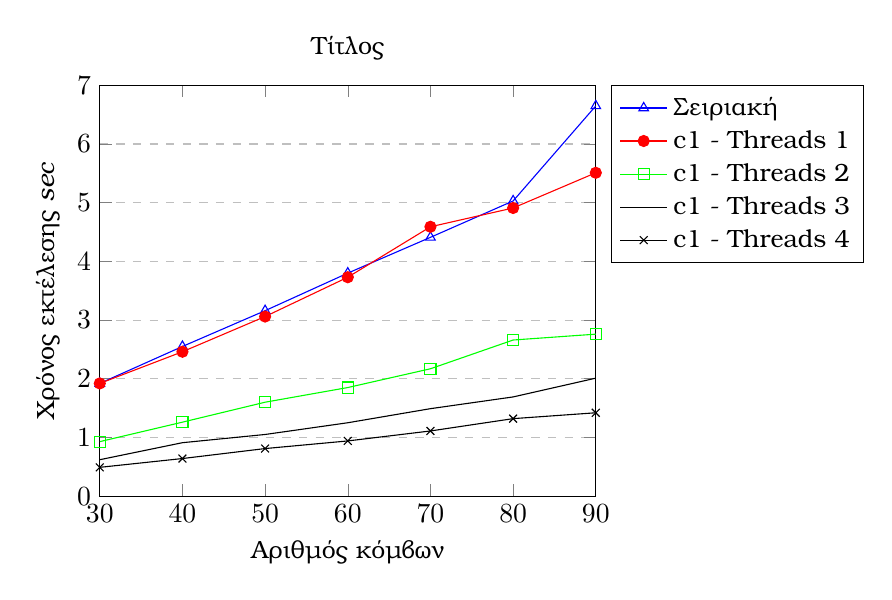
\begin{tikzpicture}
\begin{axis}[
    title={Τίτλος},
    xlabel={Αριθμός κόμβων},
    legend cell align = {left},
    ylabel={Χρόνος εκτέλεσης \emph{\en{sec}}},
    xmin=30, xmax=90,
    ymin=0, ymax=7,
    xtick={0, 30, 40, 50, 60, 70, 80, 90},
    ytick={0,1,2,3,4,5,6, 7},
    legend pos= outer north east,
    ymajorgrids=true,
    width = 0.65\textwidth,
    grid style=dashed,
]

\addplot[
    color=blue,
    mark=triangle,
    ]
    coordinates {
    (30,1.92)(40,2.55)(50,3.16)(60,3.8)(70,4.41)(80,5.03)(90,6.65)
    };
    \addlegendentry{Σειριακή}


    \addplot[
    color=red,
    mark=*,
    ]
    coordinates {
    (30,1.92)(40,2.46)(50,3.06)(60,3.73)(70,4.59)(80,4.91)(90,5.51)
    };
	\addlegendentry{\en{c1 - Threads} 1}

        \addplot[
    color=green,
    mark=square,
    ]
    coordinates {
    (30,0.928)(40,1.26)(50,1.60)(60,1.85)(70,2.17)(80,2.66)(90,2.76)
    };
	\addlegendentry{\en{c1 - Threads} 2}
            \addplot[
    color=black,
    mark=circle,
    ]
    coordinates {
    (30,0.62)(40,0.91)(50,1.05)(60,1.25)(70,1.49)(80,1.69)(90,2.01)
    };
	\addlegendentry{\en{c1 - Threads} 3}
	
            \addplot[
    color=black,
    mark=x,
	mark options={fill=white},
    ]
    coordinates {
    (30,0.49)(40,0.64)(50,0.81)(60,0.94)(70,1.11)(80,1.32)(90,1.42)
    };
	\addlegendentry{\en{c1 - Threads} 4}
\end{axis}
\end{tikzpicture}



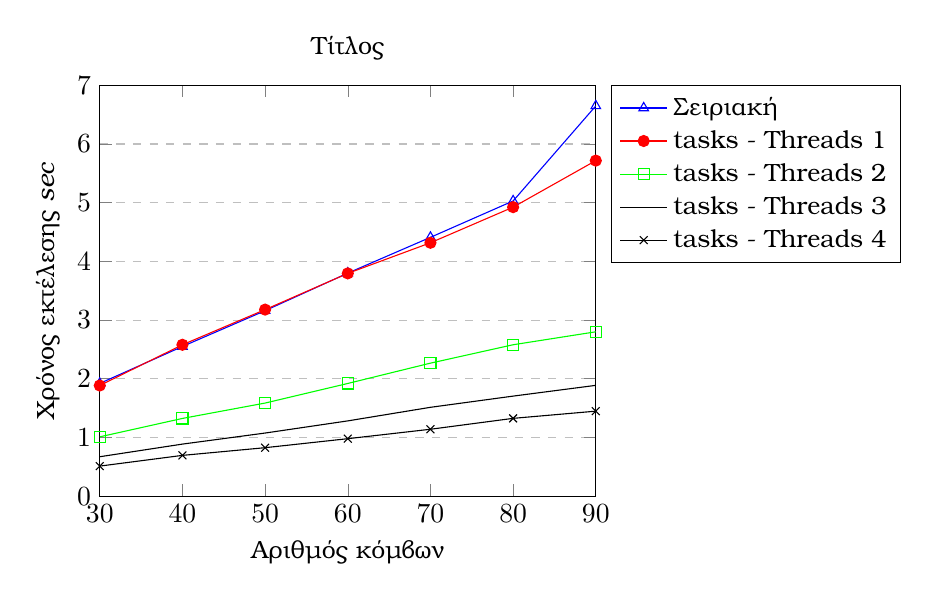
\begin{tikzpicture}
\begin{axis}[
    title={Τίτλος},
    xlabel={Αριθμός κόμβων},
    ylabel={Χρόνος εκτέλεσης \emph{\en{sec}}},
    xmin=30, xmax=90,
    ymin=0, ymax=7,
    legend cell align = {left},
    xtick={0, 30, 40, 50, 60, 70, 80, 90},
    ytick={0,1,2,3,4,5,6, 7},
    legend pos= outer north east,
    ymajorgrids=true,
    width = 0.65\textwidth,
    grid style=dashed,
]

\addplot[
    color=blue,
    mark=triangle,
    ]
    coordinates {
    (30,1.92)(40,2.55)(50,3.16)(60,3.8)(70,4.41)(80,5.03)(90,6.65)
    };
    \addlegendentry{Σειριακή}


    \addplot[
    color=red,
    mark=*,
    ]
    coordinates {
    (30,1.88436)(40,2.57883)(50,3.17825)(60,3.79555)(70,4.31703)(80,4.92457)(90,5.71748)
    };
	\addlegendentry{\en{tasks - Threads} 1}

        \addplot[
    color=green,
    mark=square,
    ]
    coordinates {
    (30,1.00991)(40,1.32349)(50,1.58554)(60,1.91951)(70,2.26585)(80,2.57923)(90,2.80001)
    };
	\addlegendentry{\en{tasks - Threads} 2}
            \addplot[
    color=black,
    mark=circle,
    ]
    coordinates {
    (30,0.670711)(40,0.886081)(50,1.07452)(60,1.28165)(70,1.51305)(80,1.70403)(90,1.88726)
    };
	\addlegendentry{\en{tasks - Threads} 3}
	
            \addplot[
    color=black,
    mark=x,
	mark options={fill=white},
    ]
    coordinates {
    (30,0.511133)(40,0.693767)(50,0.824834)(60,0.978441)(70,1.13911)(80,1.32485)(90,1.44752)
    };
	\addlegendentry{\en{tasks - Threads} 4}
\end{axis}
\end{tikzpicture}
	
\clearpage

\selectlanguage{greek}
\subsubsection{Συμπεράσματα και παρατηρήσεις}
\subparagraph{}
\clearpage
\subsection{Πρόβλημα πολλαπλασιασμού πινάκων}
\subparagraph{}
Σε αυτό το πρόβλημα γίνεται προσπάθεια επίλυσης πολλαπλασιασμού διδιάστατων πινάκων, αποτελούμενων απο τυχαίους ακεραίους:

$$C[K][M] = A[K][N] * B[N][M]$$

Για απλούστευση κώδικα, οι πίνακες που χρησιμοποιήθηκαν είναι τετραγωνικοί.

\selectlanguage{english}
\begin{lstlisting}[ tabsize = 2, basicstyle=\small, language=C++, caption={\el{Σειριακή μέθοδος πολλαπλασιασμού πινάκων}}, frame = tb]{Name}
    for (int i = 0; i < K; ++i) {
        for (int j = 0; j < M; ++j) {
            int tmp = 0;
            for (int k = 0; k < N; ++k) {
                tmp += A[i][k] * B[k][j];
            }
            C[i][j] = tmp;
        }
    }
\end{lstlisting}

\begin{lstlisting}[ tabsize = 2, basicstyle=\small, language=C++, caption={\el{Παράλληλος πολλαπλασιασμός με χρήση οδηγίας διαμοιρασμού βρόγχου}}, frame = tb]{Name}

  #pragma omp parallel for
     for (int i = 0; i < r1; ++i) {
         for (int j = 0; j < c2; ++j) {
             int tmp = 0;
             for (int k = 0; k < c1; ++k) {
                 tmp += A[i][k] * B[k][j];
             }
             C[i][j] = tmp;
         }
     }
\end{lstlisting}
\selectlanguage{greek}
Αλλη λύση του προβλήματος, είναι με διαχωρισμό των πινάκων σε υποπίνακες, και πολλαπλασιασμού των υποπινάκων ως ξεχωριστές διεργασίες\cite{examplesopm45}.

\selectlanguage{english}
\begin{lstlisting}[ tabsize = 2, basicstyle=\small, language=C++, caption={\el{Πολλαπλασιασμός πινάκων με χρήση διεργασιών (Πολλαπλασιασμός με χρήση υποπινάκων)}}, frame = tb]{Name}
void matmul(int N, int BS, int **A, int **B, int **C)
{
	int i, j, k, ii, jj, kk;
	for (i = 0; i < N; i+=BS) {
    	for (j = 0; j < N; j+=BS) {
        	for (k = 0; k < N; k+=BS) {
			// Note 1: i, j, k, A, B, C are firstprivate by default
			// Note 2: A, B and C are just pointers
			#pragma omp task private(ii, jj, kk) \
            	depend (in: A[i:BS][k:BS], B[k:BS][j:BS] ) \
            	depend (inout: C[i:BS][j:BS] )
			for (ii = i; ii < i+BS; ii++ )
				for (jj = j; jj < j+BS; jj++ )
					for (kk = k; kk < k+BS; kk++ )
						C[ii][jj] = C[ii][jj] + A[ii][kk] * B[kk][jj];
            }
        
        }
    }
}


\end{lstlisting}
\selectlanguage{greek}

\clearpage

\subsubsection{ Αποτελέσματα εκτέλεσης}
\subparagraph{}
Συγκριτικά διαγράματα εκτελέσης των τριών μεθόδων με διαφορετικά μεγέθη πινάκων αναφέρονται παρακάτω.
\selectlanguage{greek}

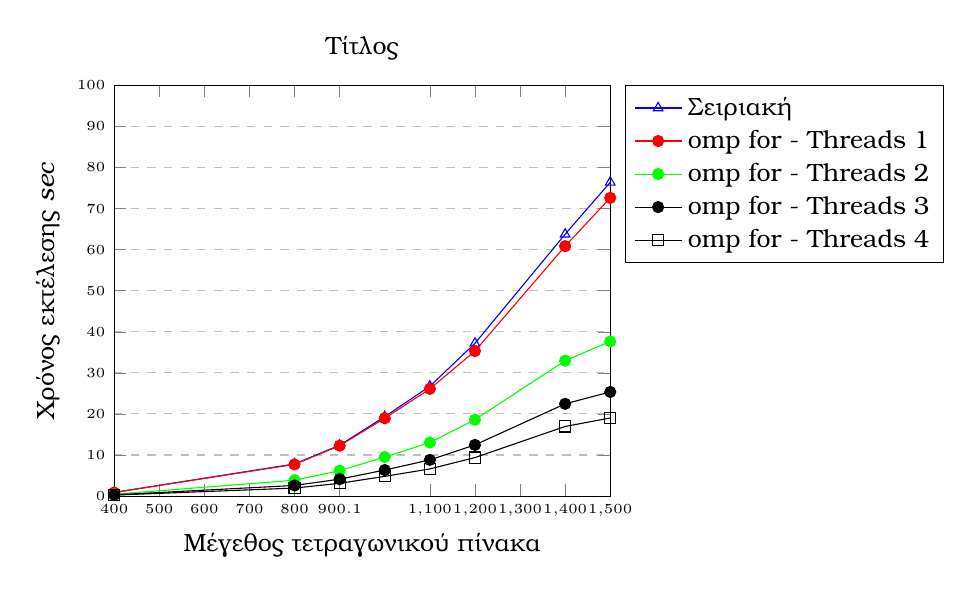
\begin{tikzpicture}
\begin{axis}[
    title={Τίτλος},
    xlabel={Μέγεθος τετραγωνικού πίνακα},
    ylabel={Χρόνος εκτέλεσης \emph{\en{sec}}},
    xmin=400, xmax=1500,
    ymin=0, ymax=100,
    legend cell align = {left},
    xtick={400, 500, 600, 700, 800, 900. 1000, 1100, 1200, 1300, 1400, 1500},
    ytick={0,10,20,30,40,50,60, 70, 80, 90, 100},
    legend pos= outer north east,
    ymajorgrids=true,
    width = 0.65\textwidth,
                       % label style={font=\small},
                    tick label style={font=\tiny} ,
    grid style=dashed,
]

\addplot[
    color=blue,
    mark=triangle,
    ]
    coordinates {
    (400,0.887962)(800,7.822277)(900,12.390038)(1000,19.337082)(1100,26.733613)(1200,37.184982)
    (1400,63.753732 )(1500,76.393354 )
    };
    \addlegendentry{Σειριακή}
    
    \addplot[
    color=red,
    mark=*,
    ]
    coordinates {
    (400,0.865326)(800,7.71938)(900,12.2757)(1000,18.947)(1100,26.1026)(1200,35.3035)
    (1400,60.8442 )(1500, 72.6156)
    };
    \addlegendentry{\en{omp for - Threads 1}}
    
        \addplot[
    color=green,
    mark=*,
    ]
    coordinates {
    (400,0.442599)(800,3.86485)(900,6.1835)(1000,9.51565)(1100,13.0426)(1200,18.5994)
    (1400,32.9676)(1500,37.6549)
    };
    \addlegendentry{\en{omp for - Threads 2}}
    
        \addplot[
    color=black,
    mark=*,
    ]
    coordinates {
    (400,0.298103)(800,2.59139)(900,4.11546)(1000,6.34454)(1100,8.81577)(1200,12.4621)
    (1400,22.4629)(1500,25.3575)
    };
    \addlegendentry{\en{omp for - Threads 3}}
            \addplot[
    color=black,
    mark=square,
    ]
    coordinates {
    (400,0.237109)(800,1.9512)(900,3.11276)(1000,4.80297)(1100,6.61739)(1200,9.37975)
    (1400,16.9502)(1500,19.0139)
    };
    \addlegendentry{\en{omp for - Threads 4}}
\end{axis}
\end{tikzpicture}

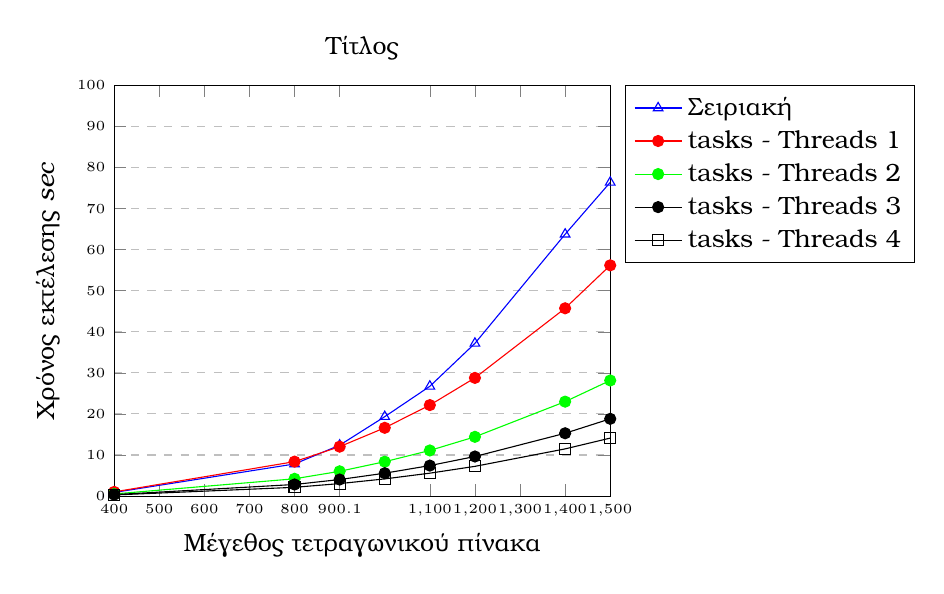
\begin{tikzpicture}
\begin{axis}[
    title={Τίτλος},
    xlabel={Μέγεθος τετραγωνικού πίνακα},
    ylabel={Χρόνος εκτέλεσης \emph{\en{sec}}},
    xmin=400, xmax=1500,
    ymin=0, ymax=100,
    legend cell align = {left},
    xtick={400, 500, 600, 700, 800, 900. 1000, 1100, 1200, 1300, 1400, 1500},
    ytick={0,10,20,30,40,50,60, 70, 80, 90, 100},
    legend pos= outer north east,
    ymajorgrids=true,
    width = 0.65\textwidth,
                       % label style={font=\small},
                    tick label style={font=\tiny} ,
    grid style=dashed,
]

\addplot[
    color=blue,
    mark=triangle,
    ]
    coordinates {
    (400,0.887962)(800,7.822277)(900,12.390038)(1000,19.337082)(1100,26.733613)(1200,37.184982)
    (1400,63.753732 )(1500,76.393354 )
    };
    \addlegendentry{Σειριακή}
    
        \addplot[
    color=red,
    mark=*,
    ]
    coordinates {
    (400,1.01848)(800,8.38982)(900,12.032)(1000,16.6239)(1100,22.1572)(1200,28.7798)
    (1400, 45.724)(1500, 56.1838)
    };
    \addlegendentry{\en{tasks - Threads 1}}
    
        \addplot[
    color=green,
    mark=*,
    ]
    coordinates {
    (400,0.520894)(800,4.2116)(900,6.03741)(1000,8.37473)(1100,11.1121)(1200,14.4275)
    (1400,22.9955)(1500,28.1515)
    };
    \addlegendentry{\en{tasks - Threads 2}}
    
        \addplot[
    color=black,
    mark=*,
    ]
    coordinates {
    (400,0.351305)(800,2.82444)(900,4.03187)(1000,5.57483)(1100,7.42902)(1200,9.6402)
    (1400,15.2952)(1500,18.8127)
    };
    \addlegendentry{\en{tasks - Threads 3}}
            \addplot[
    color=black,
    mark=square,
    ]
    coordinates {
    (400,0.272871)(800,2.13485)(900,3.04206)(1000,4.18663)(1100,5.58043)(1200,7.24081)
    (1400,11.4919)(1500,14.1197)
    };
    \addlegendentry{\en{tasks - Threads 4}}
\end{axis}
\end{tikzpicture}
\selectlanguage{greek}


\subsection{Υπολογισμού π}
\subparagraph{}

Να γράψω τα βήματα του ιντεγκρατιον και τι εινα ιτο ιντεγκρασιον.


\selectlanguage{greek}
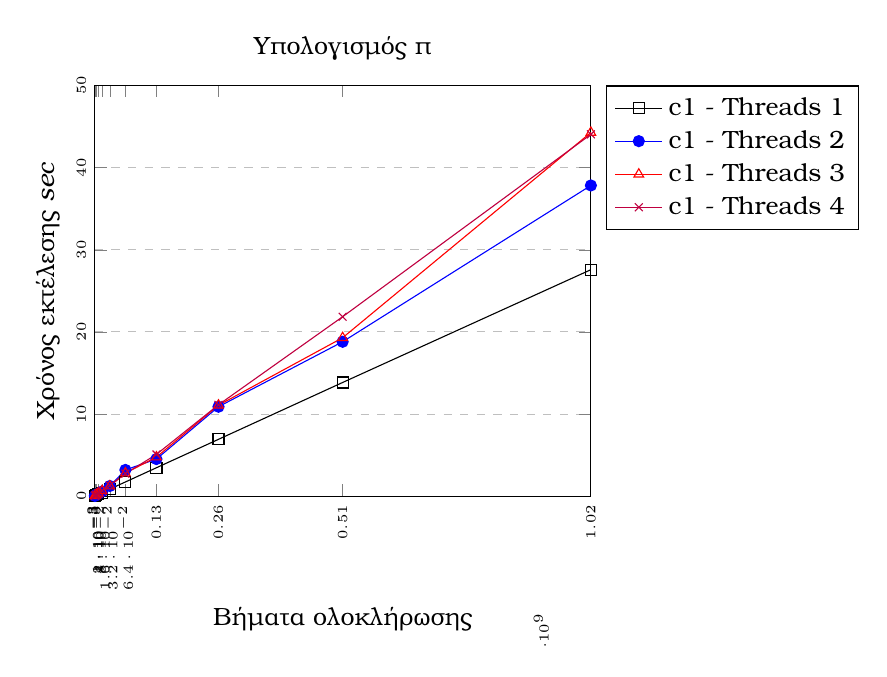
\begin{tikzpicture}
\begin{axis}[
    title={Υπολογισμός π},
    xlabel={Βήματα ολοκλήρωσης},
    ylabel={Χρόνος εκτέλεσης \emph{\en{sec}}},
    xmin=1000000, xmax=1024000000,
    ymin=0, ymax=50,
    legend cell align = {left},
    xtick={1000000, 2000000, 4000000, 8000000, 16000000, 32000000 , 64000000, 128000000, 256000000, 512000000,1024000000 },
    ytick={0,10,20,30,40,50},
    legend pos= outer north east,
    ymajorgrids=true,
    width = 0.65\textwidth,
                       % label style={font=\small},
                    tick label style={font=\tiny, rotate=90} ,
    grid style=dashed,
]
\addplot[
    color=black,
    mark=square,
    ]
    coordinates {
    (1000000,0.0338001)(2000000,0.0572331)(4000000,0.111447)(8000000,0.221375)(16000000,0.426203)(32000000,0.870774)(64000000,1.73383)(128000000,3.4648)(256000000,6.92544)(512000000,13.8453)(1024000000,27.5772)
    };
    \addlegendentry{\en{c1 - Threads 1}}
    
    \addplot[
    color=blue,
    mark=*,
    ]
    coordinates {
    (1000000,0.0405066)(2000000,0.0819236)(4000000,0.210316)(8000000,0.300327)(16000000,0.579097)(32000000,1.24199)(64000000,3.20186)(128000000,4.52216)(256000000,10.8937)(512000000,18.8005)(1024000000,37.8296)
    };
    \addlegendentry{\en{c1 - Threads 2}}
    
\addplot[
    color=red,
    mark=triangle,
    ]
    coordinates {
    (1000000,0.0436258)(2000000,0.080974)(4000000,0.175825)(8000000,0.350371)(16000000,0.664527)(32000000,1.23263)(64000000,2.80946)(128000000,4.75729)(256000000,11.0764)(512000000,19.2894)(1024000000,44.2821)
    };
    \addlegendentry{\en{c1 - Threads 3}}
    
    \addplot[
    color=purple,
    mark=x,
    ]
    coordinates {
    (1000000,0.0532062)(2000000,0.101833)(4000000,0.17677)(8000000,0.325933)(16000000,0.677992)(32000000,1.31605)(64000000,2.74918)(128000000,5.08923)(256000000,11.1267)(512000000,21.8488)(1024000000,44.0514)
    };
    \addlegendentry{\en{c1 - Threads 4}}
\end{axis}
\end{tikzpicture}


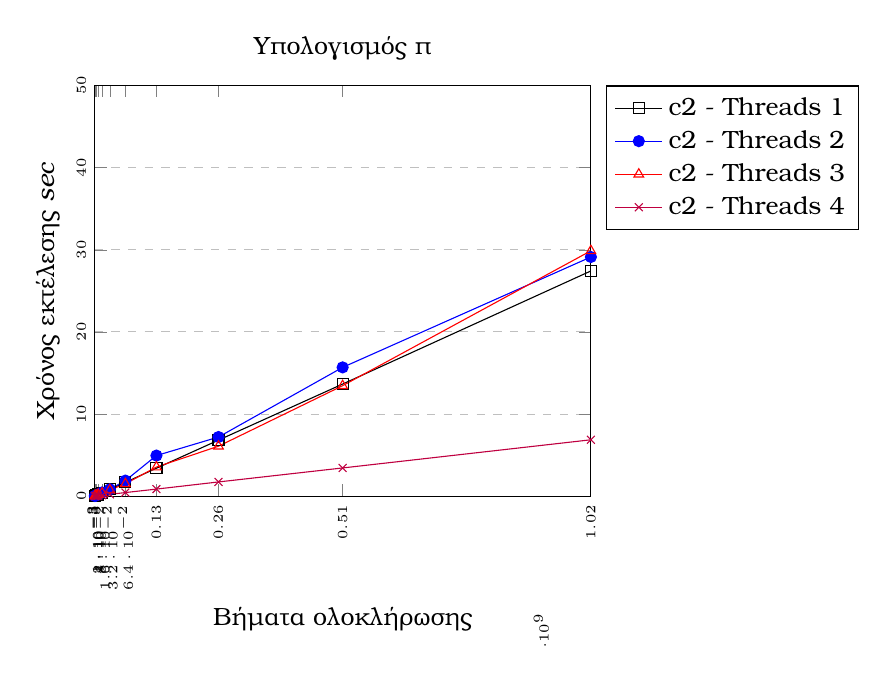
\begin{tikzpicture}
\begin{axis}[
    title={Υπολογισμός π},
    xlabel={Βήματα ολοκλήρωσης},
    ylabel={Χρόνος εκτέλεσης \emph{\en{sec}}},
    xmin=1000000, xmax=1024000000,
    ymin=0, ymax=50,
    legend cell align = {left},
    xtick={1000000, 2000000, 4000000, 8000000, 16000000, 32000000 , 64000000, 128000000, 256000000, 512000000,1024000000 },
    ytick={0,10,20,30,40,50},
    legend pos= outer north east,
    ymajorgrids=true,
    width = 0.65\textwidth,
                       % label style={font=\small},
                    tick label style={font=\tiny, rotate=90} ,
    grid style=dashed,
]
\addplot[
    color=black,
    mark=square,
    ]
    coordinates {
    (1000000,0.0308711)(2000000,0.0573471)(4000000,0.113584)(8000000,0.218868)(16000000,0.435251)(32000000,0.843545)(64000000,1.68444)(128000000,3.40944)(256000000,6.82742)(512000000,13.6523)(1024000000,27.4227)
    };
    \addlegendentry{\en{c2 - Threads 1}}
    
    \addplot[
    color=blue,
    mark=*,
    ]
    coordinates {
    (1000000,0.0317523)(2000000,0.0577772)(4000000,0.107732)(8000000,0.218209)(16000000,0.45667)(32000000,0.844152)(64000000,1.89964)(128000000,4.94725)(256000000,7.2048)(512000000,15.6844)(1024000000,29.1235)
    };
    \addlegendentry{\en{c2 - Threads 2}}
    
\addplot[
    color=red,
    mark=triangle,
    ]
    coordinates {
    (1000000,0.0310962)(2000000,0.0537551)(4000000,0.101099)(8000000,0.192268)(16000000,0.38278)(32000000,0.757889)(64000000,1.51423)(128000000,3.55208)(256000000,6.08762)(512000000,13.4538)(1024000000,29.8761)
    };
    \addlegendentry{\en{c2 - Threads 3}}
    
    \addplot[
    color=purple,
    mark=x,
    ]
    coordinates {
    (1000000,0.0159759)(2000000,0.0215767)(4000000,0.0348523)(8000000,0.0612981)(16000000,0.115281)(32000000,0.232632)(64000000,0.444231)(128000000,0.86781)(256000000,1.73724)(512000000,3.44095)(1024000000,6.86932)
    };
    \addlegendentry{\en{c2 - Threads 4}}
\end{axis}
\end{tikzpicture}

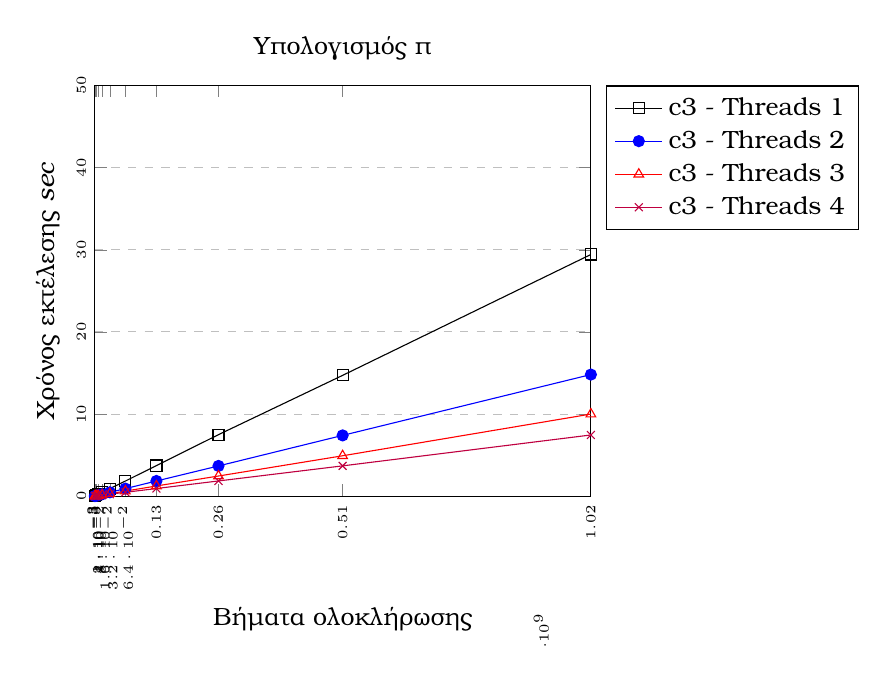
\begin{tikzpicture}
\begin{axis}[
    title={Υπολογισμός π},
    xlabel={Βήματα ολοκλήρωσης},
    ylabel={Χρόνος εκτέλεσης \emph{\en{sec}}},
    xmin=1000000, xmax=1024000000,
    ymin=0, ymax=50,
    legend cell align = {left},
    xtick={1000000, 2000000, 4000000, 8000000, 16000000, 32000000 , 64000000, 128000000, 256000000, 512000000,1024000000 },
    ytick={0,10,20,30,40,50},
    legend pos= outer north east,
    ymajorgrids=true,
    width = 0.65\textwidth,
                       % label style={font=\small},
                    tick label style={font=\tiny, rotate=90} ,
    grid style=dashed,
]
\addplot[
    color=black,
    mark=square,
    ]
    coordinates {
    (1000000,0.0341946)(2000000,0.059996)(4000000,0.120679)(8000000,0.236262)(16000000,0.477396)(32000000,0.924997)(64000000,1.84543)(128000000,3.7328)(256000000,7.49432)(512000000,14.7111)(1024000000,29.4277)
    };
    \addlegendentry{\en{c3 - Threads 1}}
    
    \addplot[
    color=blue,
    mark=*,
    ]
    coordinates {
    (1000000,0.0238432)(2000000,0.035713)(4000000,0.0669172)(8000000,0.12263)(16000000,0.238332)(32000000,0.474312)(64000000,0.925321)(128000000,1.85284)(256000000,3.6848)(512000000,7.40389)(1024000000,14.8101)
    };
    \addlegendentry{\en{c3 - Threads 2}}
    
\addplot[
    color=red,
    mark=triangle,
    ]
    coordinates {
    (1000000,0.0176296)(2000000,0.0273897)(4000000,0.0485577)(8000000,0.0817514)(16000000,0.160832)(32000000,0.315039)(64000000,0.621319)(128000000,1.2484)(256000000,2.4588)(512000000,4.92288)(1024000000,10.001)
    };
    \addlegendentry{\en{c3 - Threads 3}}
    
    \addplot[
    color=purple,
    mark=x,
    ]
    coordinates {
    (1000000,0.0155331)(2000000,0.0244363)(4000000,0.0377688)(8000000,0.0670685)(16000000,0.124106)(32000000,0.247325)(64000000,0.474941)(128000000,0.93633)(256000000,1.8583)(512000000,3.69461)(1024000000,7.45551)
    };
    \addlegendentry{\en{c3 - Threads 4}}
\end{axis}
\end{tikzpicture}


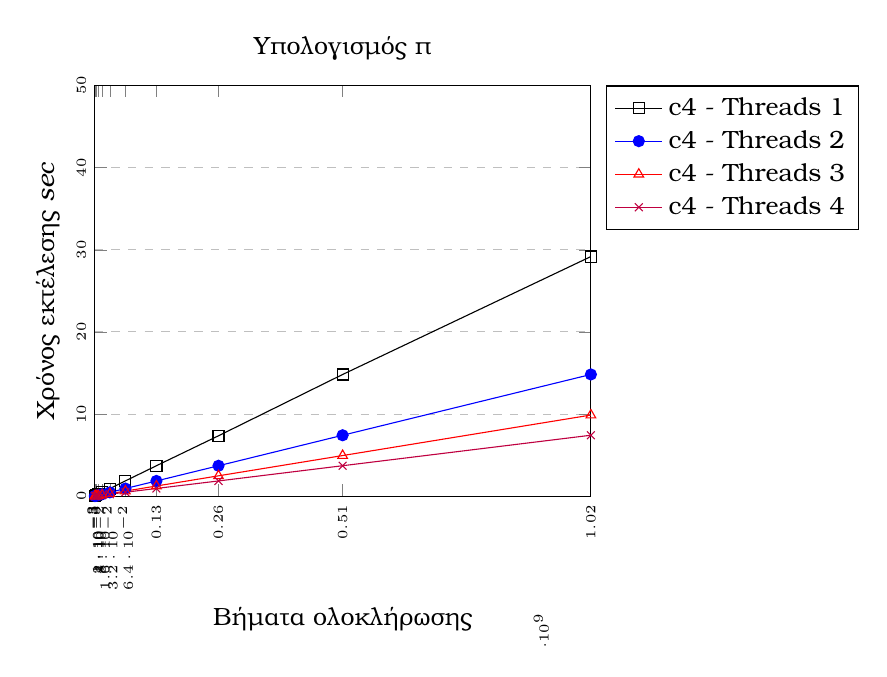
\begin{tikzpicture}
\begin{axis}[
    title={Υπολογισμός π},
    xlabel={Βήματα ολοκλήρωσης},
    ylabel={Χρόνος εκτέλεσης \emph{\en{sec}}},
    xmin=1000000, xmax=1024000000,
    ymin=0, ymax=50,
    legend cell align = {left},
    xtick={1000000, 2000000, 4000000, 8000000, 16000000, 32000000 , 64000000, 128000000, 256000000, 512000000,1024000000 },
    ytick={0,10,20,30,40,50},
    legend pos= outer north east,
    ymajorgrids=true,
    width = 0.65\textwidth,
                       % label style={font=\small},
                    tick label style={font=\tiny, rotate=90} ,
    grid style=dashed,
]
\addplot[
    color=black,
    mark=square,
    ]
    coordinates {
    (1000000,0.0326437)(2000000,0.0627669)(4000000,0.119978)(8000000,0.237184)(16000000,0.467504)(32000000,0.919998)(64000000,1.86394)(128000000,3.71113)(256000000,7.35653)(512000000,14.819)(1024000000,29.1752)
    };
    \addlegendentry{\en{c4 - Threads 1}}
    
    \addplot[
    color=blue,
    mark=*,
    ]
    coordinates {
    (1000000,0.0243332)(2000000,0.0373347)(4000000,0.0671596)(8000000,0.123871)(16000000,0.238785)(32000000,0.468718)(64000000,0.934431)(128000000,1.8579)(256000000,3.70638)(512000000,7.41984)(1024000000,14.823)
    };
    \addlegendentry{\en{c4 - Threads 2}}
    
\addplot[
    color=red,
    mark=triangle,
    ]
    coordinates {
    (1000000,0.0178636)(2000000,0.0274041)(4000000,0.0469626)(8000000,0.086801)(16000000,0.160611)(32000000,0.316492)(64000000,0.62383)(128000000,1.24284)(256000000,2.48271)(512000000,4.94991)(1024000000,9.88145)
    };
    \addlegendentry{\en{c4 - Threads 3}}
    
    \addplot[
    color=purple,
    mark=x,
    ]
    coordinates {
    (1000000,0.0157718)(2000000,0.0228653)(4000000,0.0386606)(8000000,0.0663903)(16000000,0.124964)(32000000,0.247752)(64000000,0.481567)(128000000,0.944467)(256000000,1.859)(512000000,3.71203)(1024000000,7.42446)
    };
    \addlegendentry{\en{c4 - Threads 4}}
\end{axis}
\end{tikzpicture}

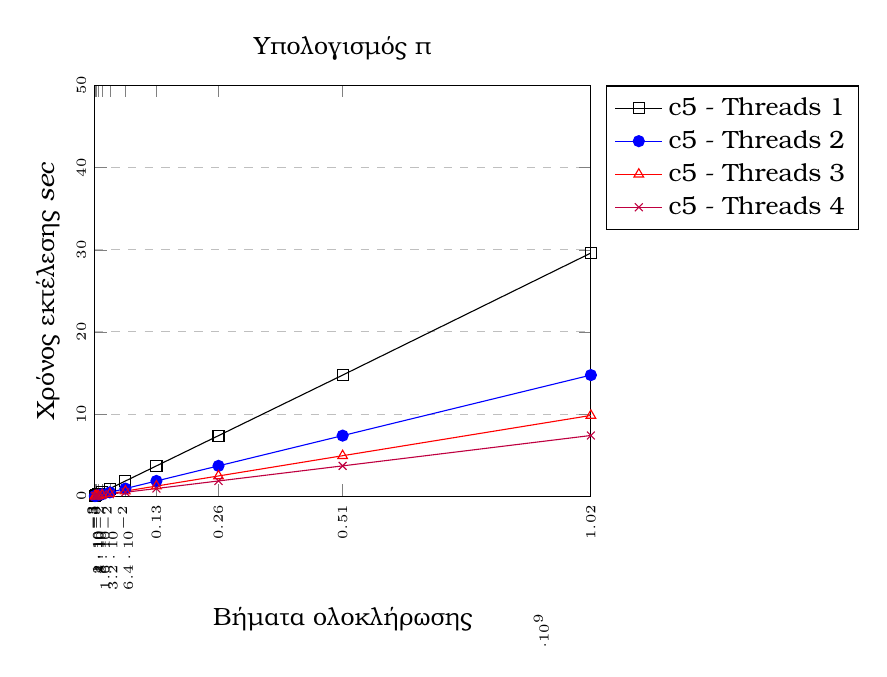
\begin{tikzpicture}
\begin{axis}[
    title={Υπολογισμός π},
    xlabel={Βήματα ολοκλήρωσης},
    ylabel={Χρόνος εκτέλεσης \emph{\en{sec}}},
    xmin=1000000, xmax=1024000000,
    ymin=0, ymax=50,
    legend cell align = {left},
    xtick={1000000, 2000000, 4000000, 8000000, 16000000, 32000000 , 64000000, 128000000, 256000000, 512000000,1024000000 },
    ytick={0,10,20,30,40,50},
    legend pos= outer north east,
    ymajorgrids=true,
    width = 0.65\textwidth,
                       % label style={font=\small},
                    tick label style={font=\tiny, rotate=90} ,
    grid style=dashed,
]
\addplot[
    color=black,
    mark=square,
    ]
    coordinates {
    (1000000,0.0339535)(2000000,0.0632102)(4000000,0.120177)(8000000,0.238885)(16000000,0.467136)(32000000,0.924733)(64000000,1.849)(128000000,3.6898)(256000000,7.37323)(512000000,14.7417)(1024000000,29.6053)
    };
    \addlegendentry{\en{c5 - Threads 1}}
    
    \addplot[
    color=blue,
    mark=*,
    ]
    coordinates {
    (1000000,0.024335)(2000000,0.0344515)(4000000,0.0675575)(8000000,0.125115)(16000000,0.238339)(32000000,0.468582)(64000000,0.928458)(128000000,1.85658)(256000000,3.69315)(512000000,7.37672)(1024000000,14.7462)
    };
    \addlegendentry{\en{c5 - Threads 2}}
    
\addplot[
    color=red,
    mark=triangle,
    ]
    coordinates {
    (1000000,0.0164176)(2000000,0.0281208)(4000000,0.0487261)(8000000,0.0858676)(16000000,0.161913)(32000000,0.315858)(64000000,0.622041)(128000000,1.23661)(256000000,2.46552)(512000000,4.92953)(1024000000,9.83403)
    };
    \addlegendentry{\en{c5 - Threads 3}}
    
    \addplot[
    color=purple,
    mark=x,
    ]
    coordinates {
    (1000000,0.0157494)(2000000,0.0247767)(4000000,0.0356085)(8000000,0.0663202)(16000000,0.131022)(32000000,0.247863)(64000000,0.478779)(128000000,0.938146)(256000000,1.85777)(512000000,3.69327)(1024000000,7.3935)
    };
    \addlegendentry{\en{c5 - Threads 4}}
\end{axis}
\end{tikzpicture}

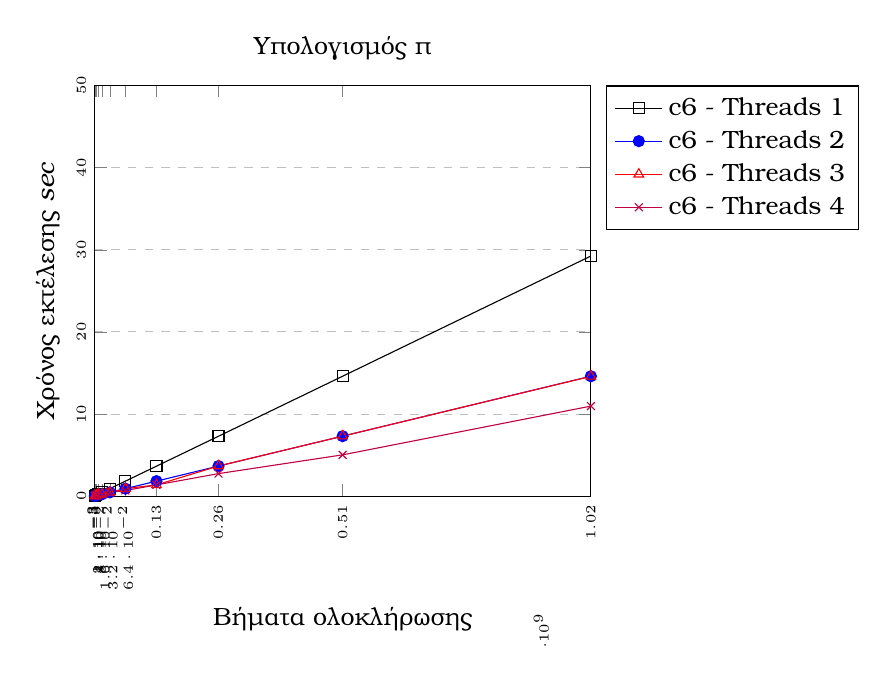
\begin{tikzpicture}
\begin{axis}[
    title={Υπολογισμός π},
    xlabel={Βήματα ολοκλήρωσης},
    ylabel={Χρόνος εκτέλεσης \emph{\en{sec}}},
    xmin=1000000, xmax=1024000000,
    ymin=0, ymax=50,
    legend cell align = {left},
    xtick={1000000, 2000000, 4000000, 8000000, 16000000, 32000000 , 64000000, 128000000, 256000000, 512000000,1024000000 },
    ytick={0,10,20,30,40,50},
    legend pos= outer north east,
    ymajorgrids=true,
    width = 0.65\textwidth,
                       % label style={font=\small},
                    tick label style={font=\tiny, rotate=90} ,
    grid style=dashed,
]
\addplot[
    color=black,
    mark=square,
    ]
    coordinates {
    (1000000,0.0336593)(2000000,0.0600598)(4000000,0.118257)(8000000,0.23635)(16000000,0.463466)(32000000,0.918388)(64000000,1.83331)(128000000,3.65506)(256000000,7.30093)(512000000,14.6071)(1024000000,29.2407)
    };
    \addlegendentry{\en{c6 - Threads 1}}
    
    \addplot[
    color=blue,
    mark=*,
    ]
    coordinates {
    (1000000,0.0355824)(2000000,0.0627649)(4000000,0.119635)(8000000,0.233565)(16000000,0.237902)(32000000,0.464477)(64000000,0.919029)(128000000,1.83531)(256000000,3.66849)(512000000,7.30996)(1024000000,14.6068)
    };
    \addlegendentry{\en{c6 - Threads 2}}
    
\addplot[
    color=red,
    mark=triangle,
    ]
    coordinates {
    (1000000,0.0346595)(2000000,0.0630393)(4000000,0.121526)(8000000,0.233586)(16000000,0.236518)(32000000,0.465431)(64000000,0.922043)(128000000,1.37825)(256000000,3.67671)(512000000,7.31318)(1024000000,14.5934)
    };
    \addlegendentry{\en{c6 - Threads 3}}
    
    \addplot[
    color=purple,
    mark=x,
    ]
    coordinates {
    (1000000,0.0349871)(2000000,0.0628435)(4000000,0.119083)(8000000,0.235015)(16000000,0.236679)(32000000,0.466)(64000000,0.694128)(128000000,1.37762)(256000000,2.75137)(512000000,5.03613)(1024000000,10.9699)
    };
    \addlegendentry{\en{c6 - Threads 4}}
\end{axis}
\end{tikzpicture}
\selectlanguage{greek}

\clearpage
\subsection{Πρόβλημα ακολουθίας \en{Fibonacci}}
\subparagraph{}
\selectlanguage{greek}


Στο παρακάτω παράδειγμα, γίνεται ο υπολογισμός αριθμών της ακολουθίας Fibonacci.

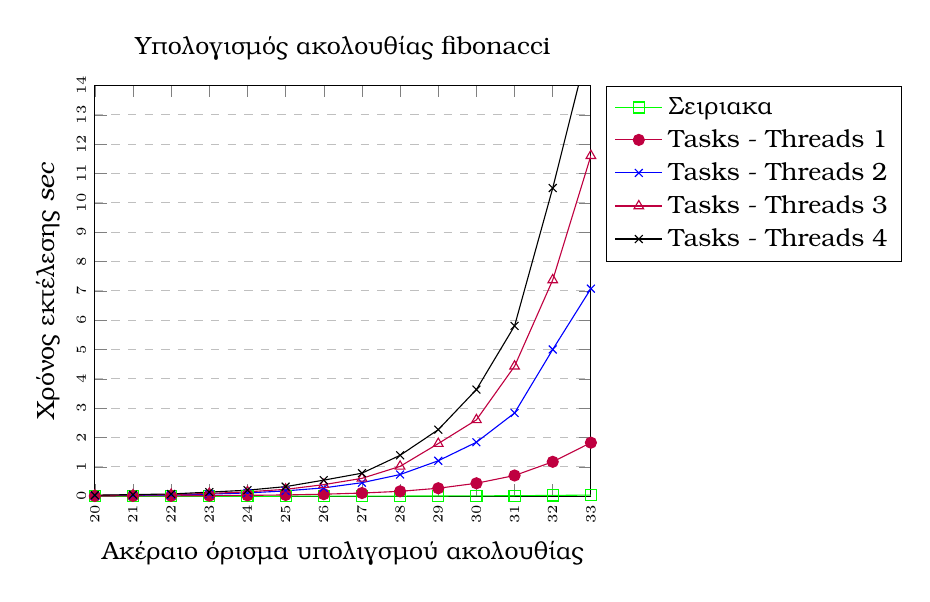
\begin{tikzpicture}
\begin{axis}[
    title={Υπολογισμός ακολουθίας \en{fibonacci}},
    xlabel={Ακέραιο όρισμα υπολιγσμού ακολουθίας},
    ylabel={Χρόνος εκτέλεσης \emph{\en{sec}}},
    xmin=20, xmax=33,
    ymin=0, ymax=14,
    legend cell align = {left},
    xtick={20, 21, 22, 23, 24, 25, 26, 27, 28, 29, 30, 31, 32, 33},
    ytick={0, 1, 2, 3, 4, 5, 6, 7, 8, 9, 10, 11, 12, 13, 14},
    legend pos= outer north east,
    ymajorgrids=true,
    width = 0.65\textwidth,
                       % label style={font=\small},
                    tick label style={font=\tiny, rotate=90} ,
    grid style=dashed,
]

    
    \addplot[
    color=green,
    mark=square,
    ]
    coordinates {
    (20,0.000122097)(21,0.000272111)(22,0.000430536)(23,0.000409333)(24,0.00113057)(25,0.00141876)(26,0.00298631)(27,0.00495223)(28,0.00562632)(29,0.00936043)(30,0.0116785)
    (31,0.0184183)(32,0.0275102)(33,0.0401246)
    };
    \addlegendentry{Σειριακα}
    
        \addplot[
    color=purple,
    mark=*,
    ]
    coordinates {
    (20,0.00890836)(21,0.0108529)(22,0.0133473)(23,0.0193422)(24,0.0294923)(25,0.0440121)(26,0.0698217)(27,0.108529)(28,0.167679)(29,0.272621)(30,0.441719)
    (31,0.706872)(32,1.1736)(33,1.82593)
    };
    \addlegendentry{\en{Tasks - Threads 1}}
    
            \addplot[
    color=blue,
    mark=x,
    ]
    coordinates {
    (20,0.0208804)(21,0.0307545)(22,0.0459824)(23,0.0724208)(24,0.112487)(25,0.18253)(26,0.285626)(27,0.461611)(28,0.739798)(29,1.20895)(30,1.84069)
    (31,2.83749)(32,5.00284)(33,7.07542)
    };
    \addlegendentry{\en{Tasks - Threads 2}}
    
                \addplot[
    color=purple,
    mark=triangle,
    ]
    coordinates {
    (20,0.0301488)(21,0.0389012)(22,0.0590625)(23,0.0946988)(24,0.149659)(25,0.235231)(26,0.394644)(27,0.609937)(28,1.01815)(29,1.79491)(30,2.60338)
    (31,4.43093)(32,7.3724)(33,11.6082)
    };
    \addlegendentry{\en{Tasks - Threads 3}}
                    \addplot[
    color=black,
    mark=x,
    ]
    coordinates {
    (20,0.0363369)(21,0.055894)(22,0.0776081)(23,0.140359)(24,0.206626)(25,0.327944)(26,0.548839)(27,0.785649)(28,1.39474)(29,2.26885)(30,3.63612)
    (31,5.80738)(32,10.5055)(33,15.6925)
    };
    \addlegendentry{\en{Tasks - Threads 4}}
\end{axis}
\end{tikzpicture}
\selectlanguage{greek}


\clearpage
While the if clause affects the task being defined by a task construct (and only
that one), the final clause affects all its descendant tasks (even if they do not have a
final clause themselves)

Η έκφραση της συνθήκης \emph{\en{if}} μιας διεργασίας, θα πρέπει να αξιολογείται ώς ψευδής ή αληθής. 
Η οδηγία των διεργασιών παρέχει μια φράση \emph{\en{if}}, που δέχεται μια έκραση ως όρισμα. Αν η έκφραση αξιολογείται ώς ψευδής, απαγορεύει η αναβολή της διεργασίας.
Ανεξαρήτου αποτελέσματος της έκφρασης, δημιουργείται πάντα ένα νέο περιβάλλον δεδομένων εργίας. Αν η έκφραση αξιολογείται ως ψευδής, δεν γίνονται όλοι οι υπολογισμοί που απετούνται για μια διεργασία αν δεν υπήρχε η φράση if, επομένως θα μπορούσαν να αποφευχθούν ορισμένα κόστη επιδόσεων.

Ως εκ τούτου η φράση \emph{\en{if}} αποτελεί λύση σε καταστάσεις, όπως οι αναδρομικοί αλγόριθμοι, όπου
το υπολογιστικό κόστος μειώνεται καθώς αυξάνεται το βάθος και το όφελος από τη δημιουργία μιας νέας διεργασίας
μειώνεται λόγω του γενικού κόστους.
Ωστόσο, για λόγους ασφαλείας \cite{parallel_dist}, οι μεταβλητές που αναφέρονται σε μια οδηγία κατασκευής διεργασιών είναι, στις περισσότερες περιπτώσεις, από προεπιλογή \emph{\en{firstprivate}}, επομένως το κόστος
της ρύθμισης περιβάλλοντος δεδομένων μπορεί να είναι το κυρίαρχο συστατικό της δημιουργίας διεργασιών.


Στην περίπτωση αληθούς έκφρασης
The scalar expression on this clause must evaluate to true or false. In the case of the latter, the encountering task is suspended and the new task is executed immediately. The parent task resumes, once the new task has completed.
This feature can be used by an implementation to improve the performance by avoiding queueing tasks that are too small.
The difference with the final clause below, is that, with the if clause, the child tasks are not affected. This is why it was not used in the example shown in Figure 3.19. Due to the nature of the quicksort algorithm, once the length of the array drops below the threshold, the length for child tasks is also below this value.



\clearpage

\section{Επίλογος}
\subparagraph{}
Εδώ συνοψίζουμε την παρουσίαση της διπλωματικής.

\subsection{Σύνοψη και συμπεράσματα}
\subparagraph{}

Εδώ συνοψίζουμε τα αποτελέσματα της διπλωματικής και περιγράφουμε τα συμπεράσματα που προέκυψαν, αρνητικά και θετικά. Επιβεβαιώνουμε τη συνεισφορά της διπλωματικής στα προβλήματα που αναφέραμε στην εισαγωγή. Τα συμπεράσματα θα πρέπει να παρουσιάζονται συστηματικά για κάθε αντικειμενικό στόχο ή υπόθεση που έχουμε κάνει.

\subsection{Όρια και περιορισμοί της έρευνας}
\subsection{Μελλοντικές Επεκτάσεις}
\subparagraph{}
Εδώ δίνουμε ιδέες για επέκταση της διπλωματικής. Αναφέρουμε ότι θα ακολουθήσει παρουσίαση μελλοντικών κατευθύνσεων έρευνας ανά θεματική περιοχή. Περιγράφουμε προβλήματα που δεν έχουν λυθεί από τις τεχνικές/μεθοδολογίες που παρουσιάσαμε στο προηγούμενο κεφάλαιο. Τα άλυτα αυτά προβλήματα, αποτελούν στην ουσία προκλήσεις για περαιτέρω έρευνα. Ακόμα καλύτερα, θα ήταν ωραία να προτείνουμε τρόπους επίλυσης των προβλημάτων αυτών έστω και ως γενική ιδέα.

\clearpage
\selectlanguage{greek}

 \selectlanguage{english}
 \bibliography{bibliogr.bib}
 \bibliographystyle{abbrv}
\end{document}